%# -*- coding: utf-8-unix -*-
%%==================================================
%% thesis.tex
%%==================================================

% 双面打印
% \documentclass[doctor, openright, twoside]{sjtuthesis}
% \documentclass[bachelor, openany, oneside, submit]{sjtuthesis}
\documentclass[master, review]{sjtuthesis}
% \documentclass[%
%   bachelor|master|doctor,	% 必选项
%   fontset=fandol|windows|mac|ubuntu|adobe|founder, % 字体选项
%   oneside|twoside,		% 单面打印,双面打印(奇偶页交换页边距,默认)
%   openany|openright, 		% 可以在奇数或者偶数页开新章|只在奇数页开新章(默认)
%   english,			% 启用英文模版
%   review,	 		% 盲审论文,隐去作者姓名、学号、导师姓名、致谢、发表论文和参与的项目
%   submit			% 定稿提交的论文,插入签名扫描版的原创性声明、授权声明 
% ]

% 逐个导入参考文献数据库
\addbibresource{bib/thesis.bib}
% \addbibresource{bib/chap2.bib}

\begin{document}

% %% 无编号内容:中英文论文封面、授权页
% %# -*- coding: utf-8-unix -*-
\title{上海交通大学学位论文 \LaTeX 模板示例文档}
\author{某\quad{}某}
\advisor{某某教授}
% \coadvisor{某某教授}
\defenddate{2014年12月17日}
\school{上海交通大学}
\institute{某某系}
\studentnumber{0010900990}
\major{某某专业}

\englishtitle{A Sample Document for \LaTeX-basedd SJTU Thesis Template}
\englishauthor{\textsc{Mo Mo}}
\englishadvisor{Prof. \textsc{Mou Mou}}
% \englishcoadvisor{Prof. \textsc{Uom Uom}}
\englishschool{Shanghai Jiao Tong University}
\englishinstitute{\textsc{Depart of XXX, School of XXX} \\
  \textsc{Shanghai Jiao Tong University} \\
  \textsc{Shanghai, P.R.China}}
\englishmajor{A Very Important Major}
\englishdate{Dec. 17th, 2014}


% \maketitle

% \makeatletter
% \ifsjtu@submit\relax
% 	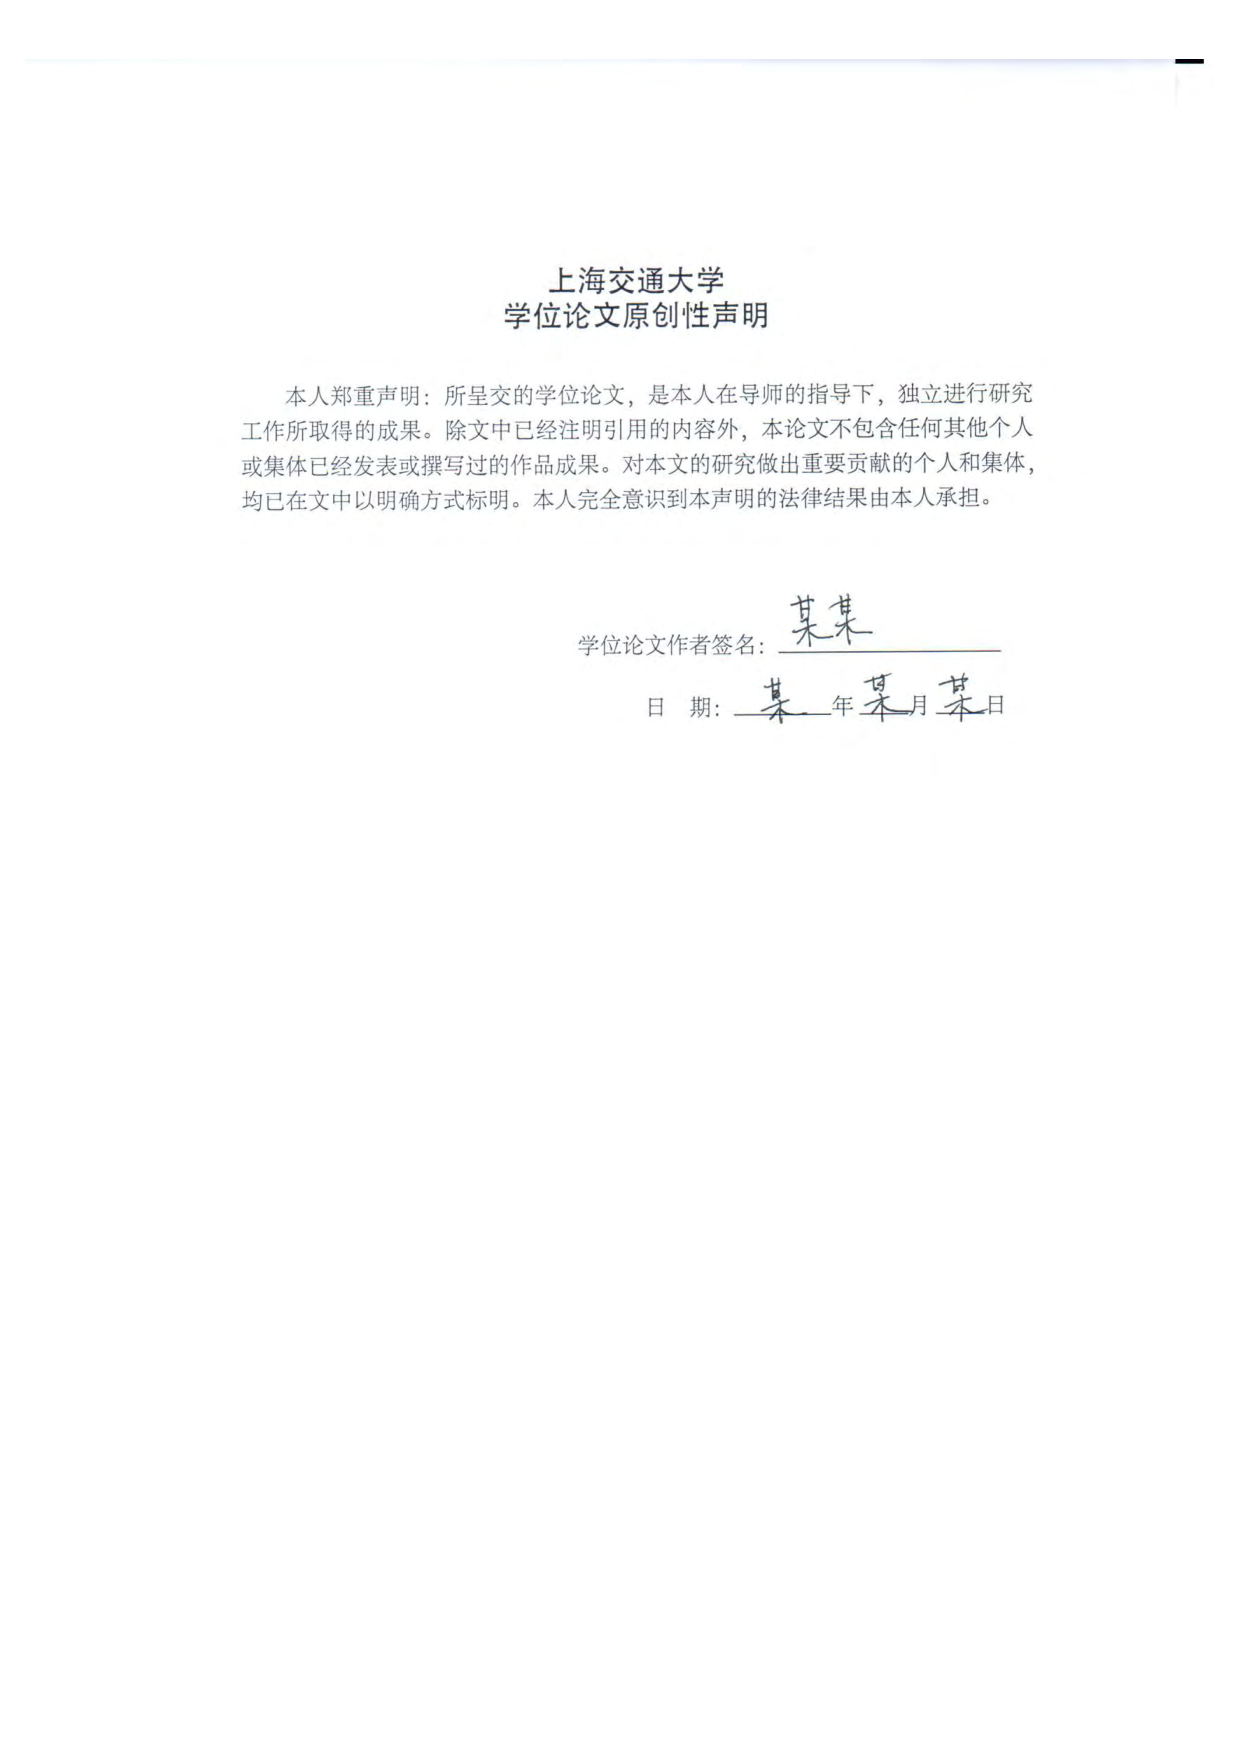
\includepdf{pdf/original.pdf}
% 	\cleardoublepage
% 	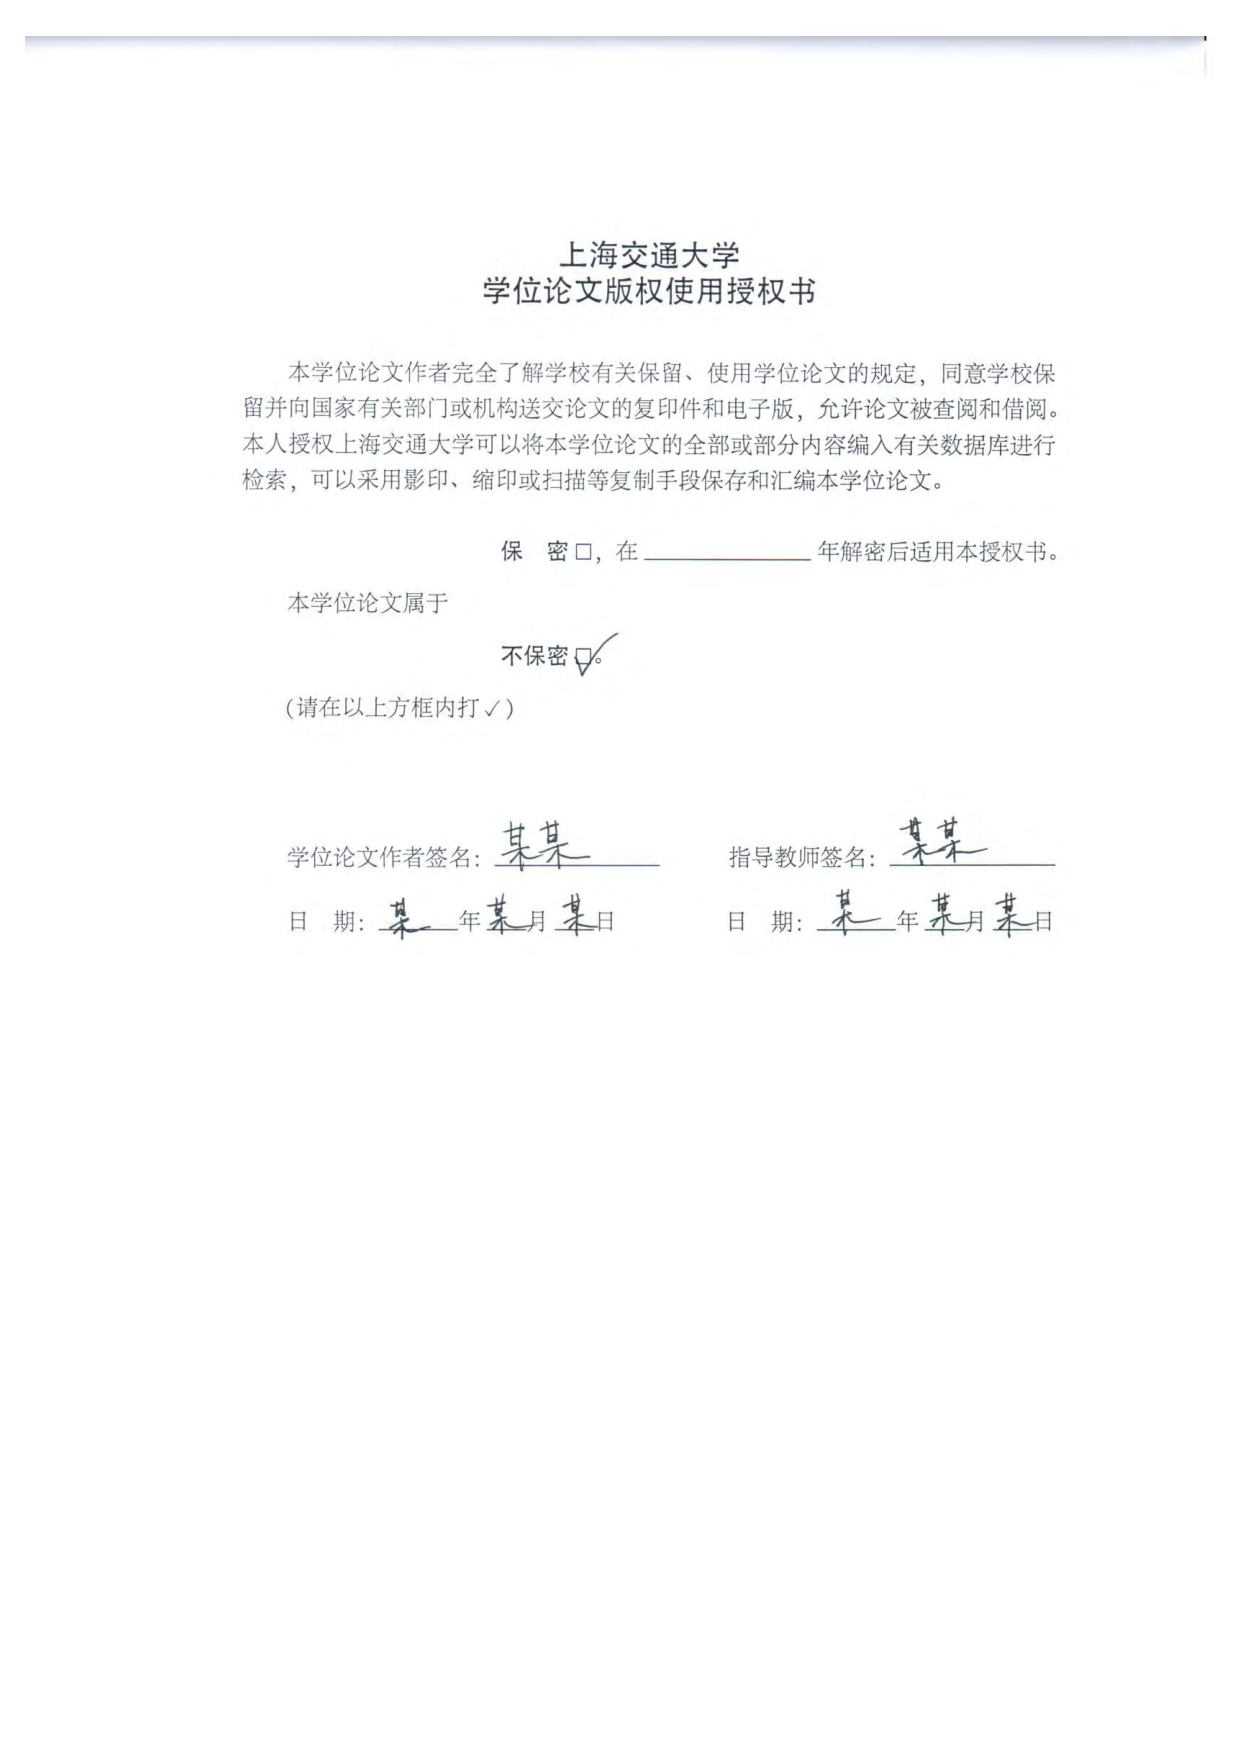
\includepdf{pdf/authorization.pdf}
% 	\cleardoublepage
% \else
% \ifsjtu@review\relax
% % exclude the original claim and authorization
% \else
% 	\makeDeclareOriginal
% 	\makeDeclareAuthorization
% \fi
% \fi
% \makeatother


% \frontmatter 	% 使用罗马数字对前言编号

%% 摘要
\pagestyle{main}
% %# -*- coding: utf-8-unix -*-
%%==================================================
%% abstract.tex for SJTU Master Thesis
%%==================================================

\begin{abstract}

上海交通大学是我国历史最悠久的高等学府之一,是教育部直属、教育部与上海市共建的全国重点大学,是国家 “七五”、“八五”重点建设和“211工程”、“985工程”的首批建设高校。经过115年的不懈努力,上海交通大学已经成为一所“综合性、研究型、国际化”的国内一流、国际知名大学,并正在向世界一流大学稳步迈进。 

十九世纪末,甲午战败,民族危难。中国近代著名实业家、教育家盛宣怀和一批有识之士秉持“自强首在储才,储才必先兴学”的信念,于1896年在上海创办了交通大学的前身——南洋公学。建校伊始,学校即坚持“求实学,务实业”的宗旨,以培养“第一等人才”为教育目标,精勤进取,笃行不倦,在二十世纪二三十年代已成为国内著名的高等学府,被誉为“东方MIT”。抗战时期,广大师生历尽艰难,移转租界,内迁重庆,坚持办学,不少学生投笔从戎,浴血沙场。解放前夕,广大师生积极投身民主革命,学校被誉为“民主堡垒”。

新中国成立初期,为配合国家经济建设的需要,学校调整出相当一部分优势专业、师资设备,支持国内兄弟院校的发展。五十年代中期,学校又响应国家建设大西北的号召,根据国务院决定,部分迁往西安,分为交通大学上海部分和西安部分。1959年3月两部分同时被列为全国重点大学,7月经国务院批准分别独立建制,交通大学上海部分启用“上海交通大学”校名。历经西迁、两地办学、独立办学等变迁,为构建新中国的高等教育体系,促进社会主义建设做出了重要贡献。六七十年代,学校先后归属国防科工委和六机部领导,积极投身国防人才培养和国防科研,为“两弹一星”和国防现代化做出了巨大贡献。

改革开放以来,学校以“敢为天下先”的精神,大胆推进改革:率先组成教授代表团访问美国,率先实行校内管理体制改革,率先接受海外友人巨资捐赠等,有力地推动了学校的教学科研改革。1984年,邓小平同志亲切接见了学校领导和师生代表,对学校的各项改革给予了充分肯定。在国家和上海市的大力支持下,学校以“上水平、创一流”为目标,以学科建设为龙头,先后恢复和兴建了理科、管理学科、生命学科、法学和人文学科等。1999年,上海农学院并入;2005年,与上海第二医科大学强强合并。至此,学校完成了综合性大学的学科布局。近年来,通过国家“985工程”和“211工程”的建设,学校高层次人才日渐汇聚,科研实力快速提升,实现了向研究型大学的转变。与此同时,学校通过与美国密西根大学等世界一流大学的合作办学,实施国际化战略取得重要突破。1985年开始闵行校区建设,历经20多年,已基本建设成设施完善,环境优美的现代化大学校园,并已完成了办学重心向闵行校区的转移。学校现有徐汇、闵行、法华、七宝和重庆南路(卢湾)5个校区,总占地面积4840亩。通过一系列的改革和建设,学校的各项办学指标大幅度上升,实现了跨越式发展,整体实力显著增强,为建设世界一流大学奠定了坚实的基础。

交通大学始终把人才培养作为办学的根本任务。一百多年来,学校为国家和社会培养了20余万各类优秀人才,包括一批杰出的政治家、科学家、社会活动家、实业家、工程技术专家和医学专家,如江泽民、陆定一、丁关根、汪道涵、钱学森、吴文俊、徐光宪、张光斗、黄炎培、邵力子、李叔同、蔡锷、邹韬奋、陈敏章、王振义、陈竺等。在中国科学院、中国工程院院士中,有200余位交大校友;在国家23位“两弹一星”功臣中,有6位交大校友;在18位国家最高科学技术奖获得者中,有3位来自交大。交大创造了中国近现代发展史上的诸多“第一”:中国最早的内燃机、最早的电机、最早的中文打字机等;新中国第一艘万吨轮、第一艘核潜艇、第一艘气垫船、第一艘水翼艇、自主设计的第一代战斗机、第一枚运载火箭、第一颗人造卫星、第一例心脏二尖瓣分离术、第一例成功移植同种原位肝手术、第一例成功抢救大面积烧伤病人手术等,都凝聚着交大师生和校友的心血智慧。改革开放以来,一批年轻的校友已在世界各地、各行各业崭露头角。

截至2011年12月31日,学校共有24个学院/直属系(另有继续教育学院、技术学院和国际教育学院),19个直属单位,12家附属医院,全日制本科生16802人、研究生24495人(其中博士研究生5059人);有专任教师2979名,其中教授835名;中国科学院院士15名,中国工程院院士20名,中组部“千人计划”49名,“长江学者”95名,国家杰出青年基金获得者80名,国家重点基础研究发展计划(973计划)首席科学家24名,国家重大科学研究计划首席科学家9名,国家基金委创新研究群体6个,教育部创新团队17个。

学校现有本科专业68个,涵盖经济学、法学、文学、理学、工学、农学、医学、管理学和艺术等九个学科门类;拥有国家级教学及人才培养基地7个,国家级校外实践教育基地5个,国家级实验教学示范中心5个,上海市实验教学示范中心4个;有国家级教学团队8个,上海市教学团队15个;有国家级教学名师7人,上海市教学名师35人;有国家级精品课程46门,上海市精品课程117门;有国家级双语示范课程7门;2001、2005和2009年,作为第一完成单位,共获得国家级教学成果37项、上海市教学成果157项。

\keywords{\large 上海交大 \quad 饮水思源 \quad 爱国荣校}
\end{abstract}

\begin{englishabstract}

An imperial edict issued in 1896 by Emperor Guangxu, established Nanyang Public School in Shanghai. The normal school, school of foreign studies, middle school and a high school were established. Sheng Xuanhuai, the person responsible for proposing the idea to the emperor, became the first president and is regarded as the founder of the university.

During the 1930s, the university gained a reputation of nurturing top engineers. After the foundation of People's Republic, some faculties were transferred to other universities. A significant amount of its faculty were sent in 1956, by the national government, to Xi'an to help build up Xi'an Jiao Tong University in western China. Afterwards, the school was officially renamed Shanghai Jiao Tong University.

Since the reform and opening up policy in China, SJTU has taken the lead in management reform of institutions for higher education, regaining its vigor and vitality with an unprecedented momentum of growth. SJTU includes five beautiful campuses, Xuhui, Minhang, Luwan Qibao, and Fahua, taking up an area of about 3,225,833 m2. A number of disciplines have been advancing towards the top echelon internationally, and a batch of burgeoning branches of learning have taken an important position domestically.

Today SJTU has 31 schools (departments), 63 undergraduate programs, 250 masters-degree programs, 203 Ph.D. programs, 28 post-doctorate programs, and 11 state key laboratories and national engineering research centers.

SJTU boasts a large number of famous scientists and professors, including 35 academics of the Academy of Sciences and Academy of Engineering, 95 accredited professors and chair professors of the "Cheung Kong Scholars Program" and more than 2,000 professors and associate professors.

Its total enrollment of students amounts to 35,929, of which 1,564 are international students. There are 16,802 undergraduates, and 17,563 masters and Ph.D. candidates. After more than a century of operation, Jiao Tong University has inherited the old tradition of "high starting points, solid foundation, strict requirements and extensive practice." Students from SJTU have won top prizes in various competitions, including ACM International Collegiate Programming Contest, International Mathematical Contest in Modeling and Electronics Design Contests. Famous alumni include Jiang Zemin, Lu Dingyi, Ding Guangen, Wang Daohan, Qian Xuesen, Wu Wenjun, Zou Taofen, Mao Yisheng, Cai Er, Huang Yanpei, Shao Lizi, Wang An and many more. More than 200 of the academics of the Chinese Academy of Sciences and Chinese Academy of Engineering are alumni of Jiao Tong University.

\englishkeywords{\large SJTU, master thesis, XeTeX/LaTeX template}
\end{englishabstract}



% %% 目录、插图目录、表格目录
% \tableofcontents
% \listoffigures
% \addcontentsline{toc}{chapter}{\listfigurename} %将插图目录加入全文目录
% \listoftables
% \addcontentsline{toc}{chapter}{\listtablename}  %将表格目录加入全文目录
% \listofalgorithms
% \addcontentsline{toc}{chapter}{\listalgorithmname}

% %# -*- coding: utf-8-unix -*-
\begin{nomenclaturename}
\label{chap:symb}

\begin{longtable}{rl}
$\epsilon$     & 介电常数 \\
 $\mu$ 		& 磁导率 \\
 $\epsilon$     & 介电常数 \\
 $\mu$ 		& 磁导率 \\
 $\epsilon$     & 介电常数 \\
 $\mu$ 		& 磁导率 \\
 $\epsilon$ 	& 介电常数 \\
 $\mu$ 		& 磁导率 \\
 $\epsilon$     & 介电常数 \\
 $\mu$ 		& 磁导率 \\
 $\epsilon$     & 介电常数 \\
 $\mu$ 		& 磁导率 \\
 $\epsilon$     & 介电常数 \\
 $\mu$ 		& 磁导率 \\
 $\epsilon$ 	& 介电常数 \\
 $\mu$ 		& 磁导率 \\
 $\epsilon$     & 介电常数 \\
 $\mu$ 		& 磁导率 \\
 $\epsilon$     & 介电常数 \\
 $\mu$ 		& 磁导率 \\
 $\epsilon$     & 介电常数 \\
 $\mu$ 		& 磁导率 \\
 $\epsilon$ 	& 介电常数 \\
 $\mu$ 		& 磁导率 \\
 $\epsilon$     & 介电常数 \\
 $\mu$ 		& 磁导率 \\
 $\epsilon$     & 介电常数 \\
 $\mu$ 		& 磁导率 \\
 $\epsilon$     & 介电常数 \\
 $\mu$ 		& 磁导率 \\
 $\epsilon$ 	& 介电常数 \\
 $\mu$ 		& 磁导率 \\
 $\epsilon$     & 介电常数 \\
 $\mu$ 		& 磁导率 \\
 $\epsilon$     & 介电常数 \\
 $\mu$ 		& 磁导率 \\
 $\epsilon$     & 介电常数 \\
 $\mu$ 		& 磁导率 \\
 $\epsilon$ 	& 介电常数 \\
 $\mu$ 		& 磁导率 \\
 $\epsilon$     & 介电常数 \\
 $\mu$ 		& 磁导率 \\
 $\epsilon$     & 介电常数 \\
 $\mu$ 		& 磁导率 \\
 $\epsilon$     & 介电常数 \\
 $\mu$ 		& 磁导率 \\
 $\epsilon$ 	& 介电常数 \\
 $\mu$ 		& 磁导率 \\
 $\epsilon$     & 介电常数 \\
 $\mu$ 		& 磁导率 \\
 $\epsilon$     & 介电常数 \\
 $\mu$ 		& 磁导率 \\
 $\epsilon$     & 介电常数 \\
 $\mu$ 		& 磁导率 \\
\end{longtable}

\end{nomenclaturename}
 % 主要符号、缩略词对照表

% \mainmatter	% 使用阿拉伯数字对正文编号

%% 正文内容
\pagestyle{main}
% %# -*- coding: utf-8-unix -*-
%%==================================================
%%==================================================

\chapter{绪论}
% \label{chap:intro}

\section{研究背景和意义}
一般在传统的医疗诊断和治疗方案决策的过程中,医生一般先要求病人进行详细全面的查体。这里查体的结果被视作一系列针对病人的理化指标。根据这些理化指标,医生再结合病人的临床病史,病人当前的状态,医生的专业知识与临床经验以及制定好的相关治疗规范或治疗手册对病人的疾病状态做进一步评估并给出合理的治疗方案。

大多数情况下病人的状态都可以用医学或者生物学的术语作准确地描述,医生也可以根据自己的知识作出较为准确的判断。对于许多典型的病例,医疗手册中可以找出符合的最优治疗方案,如果这个过程能够自动化,便可以极大程度上提升医生诊断的工作效率。但事实上很多病例并没有完美匹配医疗手册中的规则,这种情况下对病例情况的判断很大程度上依赖于医生自身的水平,具有较大的主观因素:对于一个刚刚完成职业规范化培训的医生,他的临床经验可能比较欠缺;而对于一个从医数十载的专家,他的技术可能极为精湛。考虑到医生的水平参差不齐,以及医生思考问题的角度可能不尽相同,不同的医生对同一个病例可能持有不同的态度,即每个医生心中对同一个病例的最佳治疗方案可能大相径庭。

与此同时,现代医学飞速发展,医学中各个分支领域的划分越来越细,各个方向的知识越来越深入,一个专攻某个领域的专家由于知识面相对地狭窄,因而不能凭借一己之力同时兼顾病患自身的其他方面的因素,这势必造成对病患的诊断有一定的片面性。这种情况下,多学科综合治疗(Mulity-Disciplinary Treatment,简称MDT)的概念\cite{Taylorc951}应运而生。多学科治疗是一种组织多学科协作诊治病情的形式,即由来自医院放射科、病理科、检验科、心电图、普外科等相关科室,甚至包括医联体内其他外部专家组成工作组,针对某一疾病,通过会诊方式提出适合患者的最佳治疗方案并多学科联合执行。主要针对肿瘤、疑难复杂疾病、多系统多器官疾病等。MDT综合了不同医疗领域专家的共同智慧从而保证高质量的诊治建议和最佳的治疗计划,避免过度诊疗和误诊误治,使病人受益最大化。

随着计算机科学与软件工程的发展,为了支持多学科综合治疗会议的展开,决策支持系统(Decision Support system,简称DSS)作为一个高效的工具,曾一度被不同学科的科研工作者所重视\cite{Filip2017}。智能决策系统的出现,使得高效的,大规模的多学科治疗案例得以实施。该系统的意义在于整合医疗资源,维护医疗决策过程,并总结相关知识反馈给医生,辅助医生来做判断与决策。以多学科治疗为目的的决策支持系统简称MDTDSS。智能决策系统有两大方向,分别是基于规则的系统和基于历史案例的系统。

基于规则的系统主要利用到了知识表示方法中将规则符号化的方法\cite{Ligêza2006}。该方法将规则抽象化成逻辑公式,将病人的各种指标作为输入,推导出正确的结果。这里的规则一般来源于许多医疗机构发布并使用的权威医学指南,例如国家综合癌症治疗网络(National Comprehensive Cancer Network,简称NCCN)\cite{Mohler2010The}。但是,这些指南建议的治疗方案通常是粗略的,例如可以根据病人的情况推导出该病人需要化疗却无法推导出需要哪种类型的化疗。另外,对于有些特殊的病例,并没有匹配治疗指南中的某个规则,则如果把这样的病例作为输入,系统根本无法得到一个结果。

另一个方向是基于历史病例数据的决策支持系统。基于历史病例的决策也称作基于案例的推理,对它最早的研究发生在二十世纪七十年代后期\cite{Schank1988SCRIPTS,Schank1982Dynamic}。这样的系统维护了一个供多学科团队讨论的平台,在该平台上,多学科团队的诸位专家对同一个病例多次发表意见。这些意见最终由专人进行汇总,采用投票的方式决定该病人的最终治疗方案。图\ref{fig:ch1-1}展示了某决策支持系统的多学科团队讨论模块。整个讨论过程分为三个步骤:初次投票环节,决议投票环节以及决策环节。\textbf{在初次投票环节,}医生根据病人的情况以及自己的专业知识与经验,互相独立地为病人选择一个合理的化疗方案。在该环节,多学科团队中的各个医生无法知道其他医生的意见\textbf{在决议投票环节,}医生参考其他医生对该病例的意见,可以对自己在第一轮投票的结果进行修改,或者继续坚持自己在前一轮做出的决定。\textbf{在决策环节,}投票负责人汇总决议投票的结果,以少数服从多数的方式,决定病人的最佳化疗方案。如图\ref{fig:ch1-1}所示的案例中,在决议投票之后,共有11位医生为该病人选择了EC-T方案,数量最多。因此该病人最终的化疗方案被制定为EC-T。这样一个讨论过程中,可以挖掘的知识主要有以下三个方面:
\begin{enumerate}
  \item 每位医生在初次投票中对病例情况做出的独立判断
  \item 每位医生在决议投票中对病例情况的判断发生变化的情况
  \item 该病人对应的最佳治疗方案
\end{enumerate}
这样的基于历史病例数据的决策支持系统,通过维护一个又一个对病例的讨论过程,并将讨论数据做持久化处理,可以构造出一个完整的关于疾病治疗方案的知识库。近年来,人工智能技术越来越多的得到人们的重视,人工智能与机器学习的相关算法已经深入到包括金融,生活,出行等诸多领域。将人工智能算法应用于病例知识库,对上述三种知识加以总结与分析,可以对病人的最佳治疗方案进行推荐,并把推荐结果反馈给医生,帮助医生更好的做出判断。这对于整合医疗资源与医学知识,补充医生知识与经验的缺陷以及实现精准医疗、高效医疗有重要的意义。

此外,针对基于历史病例数据的决策支持系统的本质是将待推荐病例与病例数据库中的已有知识相对比并作出相应的判断。这其中中所使用的相关推荐算法,一旦效果显著,很可能被大规模推广与使用。这样的系统可能具有较高的QPS(Queries-per-second,每秒查询率)与DAU(Daily Active User,日活跃用户数量)并且拥有相当大规模的病例数据库。同一时刻可能有多位用户并发地访问该系统,并希望系统针对某个病人,根据病理数据库中的知识获得其推荐的治疗方案。巨大的数据量与有限的算力资源之间的矛盾必然将导致推荐的时延显著增加。如何优化推荐算法以减小问题的规模,如何折中算法的复杂度与推荐结果的准确率,也是本文关注的另一个重点。

综上,本文以医疗方案的基本推荐方法为出发点,先后介绍基于规则和基于历史数据的医疗方案推荐方法,并提出了相应的优化方法;之后,本文以专家的投票数据为基础,对历史病例数据做进一步挖掘以提升推荐的性能;然后,考虑到这样的方法落地并被大规模使用之后,推荐的时延和算法的问题规模可能带来的瓶颈问题,本文提出了折中相应算法复杂度与推荐准确率的方法。在最后,本文将详细介绍相应的系统实现。
\begin{figure}[!htp]
  \centering
  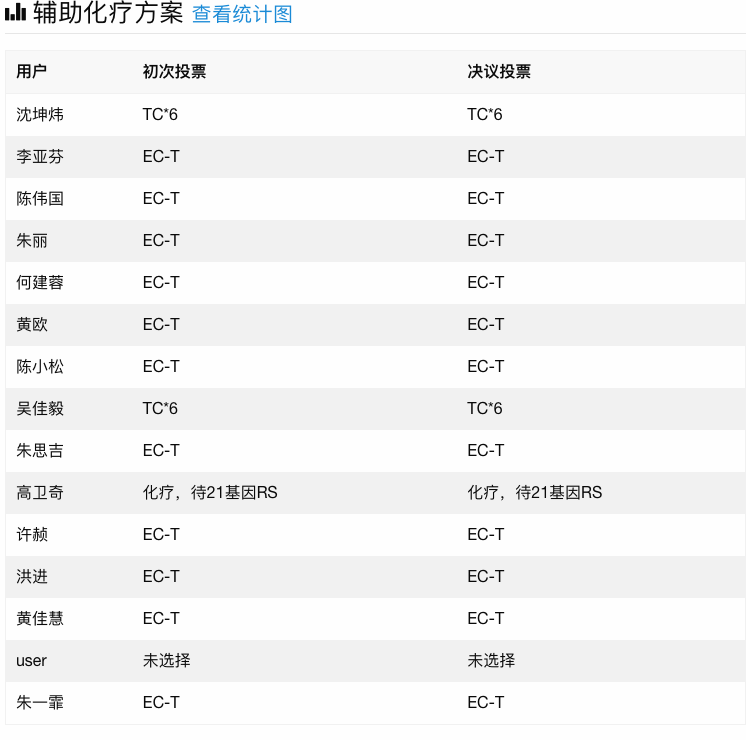
\includegraphics[width=10cm,height=12cm]{figure/ch1-fig1.png}
  \bicaption[某决策支持系统的多学科团队讨论结果]
    {某决策支持系统的多学科团队讨论结果}
    {the result of the discussion part of one MADTDSS}
  \label{fig:ch1-1}
\end{figure}

\section{国内外研究现状}

近年来,将计算机科学方法应用于治疗方案推荐一度成为科研人员的研究热点。其中提出的医疗方案推荐方法大致可以分为两个方向,分别是基于规则的推荐方法以及基于历史数据的推荐方法。本节将先后探讨基于规则的医疗推荐方法的研究现状,基于历史数据的医疗推荐方法的研究现状以及决策支持系统的研究现状。

\subsection{基于规则的医疗推荐方法}

处理诸如心力衰竭,糖尿病和慢性阻塞性肺疾病,癌症等慢性疾病是医疗中的主要问题。医学指南一般是指由一些权威医疗机构的医疗委员会的专家成员制定的,所有医师都应该遵循的,主要用于管理慢性疾病的标准方法。这些准则通常由一系列
根据患者信息提出建议的复杂规则组成。一般医疗指南都具有较长的篇幅与复杂的逻辑。比如针对慢性心力衰竭的医疗指南有80页。由于其复杂性,通常这些准则要么被忽略,要么根本不遵守,这可能导致不良的医疗实践。为了解决这一问题,在2016年,Chen Zhuo等人在文献\parencite{Chen2016A}之中描述了一种用于CHF管理的医生咨询系统,该系统使用答案集编程为CHF的整个临床实践指南进行编码。所使用的方法基于开发推理模板(即知识图谱),并使用这些模式将CHF的临床指南系统编码为ASP规则。知识图谱的使用极大地简化了系统的开发。当患者的状态和各种理化指标给定后,即使信息不完整有缺失,系统也可以像医生一样给出治疗建议。该系统的成功实践有两个明显的意义:1)该系统的成功实践表明高度复杂的准则可以成功地编码为ASP规则,2)该系统开发出一系列知识模式,这些模式有助于对以自然语言表达的知识进行编码,并可以用于其他应用领域。

对慢性疾病进行有效的临床管理有时还需要一系列治疗,每种治疗均应适应个体反应,因此需要在个人临床护理的整个过程中做出多种治疗决定。在2011年,Daniel Almirall等人提出了自适应治疗策略(adaptive treatment strategies,简称ATS)\cite{Daniel2012Designing}。ATS使得这样一系列的治疗规则化。ATS通过“关键规则”来实现个性化治疗。“关键规则”主要定义了是否,如何,以及何时改变治疗的方式与强度。关键决策的例子包括最初提供哪种治疗,等待初始治疗多长时间,如何确定初始治疗是否有效,以及如果初始治疗可以提供下一个治疗治疗有效或无效。每个关键决策的治疗方法可能包括药物,行为治疗干预,或两者结合。ATS将患者的治疗状况最为输入,将推荐的该阶段的治疗方法作为输出。为了将ATS各个阶段的最优化输出组合成为一套最优的治疗方案,文献\parencite{Daniel2012Designing}又提出了连续性多次分配实验(Sequential multiple assignment randomized trials,简称SMART)。SMART的关键特征是,它允许研究者通过使用随机数据,以原则性方式评估治疗的时机,顺序和对ATS的决策结果做出适应性选择。2016年,为了评估使用ATS和SMART对青少年抑郁症治疗的可行性,Gunlicks-Stoessel等人使用4条ATS展开了临床试验\cite{Gunlicks2017A};并对32名青少年进行了为期16周的连续性多次分配实验(SMART),初步研究的结果对全尺寸SMART提出了更多的研究问题。


\subsection{基于历史数据的医疗推荐方法}
针对基于历史病例数据的决策支持系统的本质是将待推荐病例与病例数据库中的已有知识相对比并作出相应的判断。由于复杂的疾病和药物依赖性以及药物不良相互作用的潜在风险,长期以来,对具有多种并发症的患者进行治疗一直是一个难题。不同于基于难以使用的高度复杂的规则的医疗推荐方法与基于简单统计模型的方法,Yutao Zhang等人在2017年提出了LEAP算法\cite{Zhang2017LEAP},该算法将医疗推荐分解为一系列决策过程以自动确定合适的药物数量。在文献\parencite{Zhang2017LEAP}中,循环解码器用于捕获标签实例映射的标签相关性,强化学习的相关方法用于对模型参数进行相关微调,以确保结果的完整性与准确性。文献\parencite{Zhang2017LEAP}创新性地提出外部临床知识纳入强化奖励的设计中,以有效防止产生不利的药物组合。在真实世界的电子健康记录数据集上进行了定量实验和定性案例研究表明,LEAP算法有效地消除了推荐治疗组中99.8%的不良药物相互作用。

在文献\parencite{Zhang2017iDoctor}中,介绍了一种名为iDoctor的新型医疗保健推荐系统,该系统基于混合矩阵分解方法。 iDoctor在以下方面与先前的工作有所不同:(1)用户评论的情感偏移可以通过情感分析来揭示,并可以用来修改原始用户评分; (2)通过Latent Dirichlet Allocation提取用户偏好和医生特征,并将其合并到常规矩阵分解中。 献\parencite{Zhang2017iDoctor}使用实际数据集将iDoctor与以前的医疗保健推荐方法进行了比较。 实验结果表明,iDoctor提供了更高的预测评分,并显着提高了医疗保健推荐的准确性。

文献\parencite{Thong2015HIFCF}考虑了将直觉模糊集(IFS)和推荐系统(RS)集成到所提出的方法中,并提出了一种新颖的直觉模糊推荐系统(IFRS)。与仅在传统模糊集或推荐系统上构建的相关方法相比,IFRS的预测精度更高。在观察到通过整合模糊聚类方法指定的聚类患者的可能性信息可以增强IFRS相似度计算的基础上,文献\parencite{Thong2015HIFCF}还提出了图像模糊聚类与直觉模糊之间的一种新型混合模型:HIFCF(混合直觉模糊协作过滤)。实验结果表明,HIFCF比IFCF具有更好的准确性。

2014年Pradhan等人\cite{Pradhan2014Improving}引入了一种创新的基于信任的信息模型来评估那些牙科相关评论以及调查中患者的主观因素。该模型评估了4个信任成分:上下文,关系,声誉和性格分析。使用此模型以及从社交网络中提取的信息对牙医和患者的关系进行剖析。使用从在线牙科评论获得的主观素质对牙医进行剖析,并使用从580名参与者中收集的调查结果等主观信息对患者进行剖析,例如个体对牙医的恐惧程度和人格特质。研究的结果可用于定义一套规则,以改善牙科保健推荐系统中患者和牙医之间的匹配程度。


\subsection{决策支持系统}
对决策支持系统(Decision Support system,简称DSS)的研究最早可以追溯到10年以前\cite{Filip2017}。本节将近十年以来各个领域的科研工作者对决策支持系统所做的研究进行总结,将其大致分为以下五种类型:

\begin{itemize}
\item \textbf{基于模型的DSS。}

基于模型的DSS以一个简单的数学模型为系统的核心。这种系统的着眼点主要放在如何访问与操作模型上。基于模型的DSS一般根据用户输入的数据以及用户对系统的相关配置为用户的决策提供帮助,但是一般而言,系统的数据量不大,不需要规模庞大的数据库。
\item \textbf{基于通信的DSS。}

基于通信的DSS利用诸如RPC协议\cite{Srinivasan1995RPC}等网络通信技术来促进系统中不同服务之间的协作以提升系统的性能。这样的系统以网络与通信技术为核心。上世纪后期,一部分工程师设计了群体DSS以支持群体性质的决策任务\cite{Turoff1982Computer}。之后又出现了一系列基于通信技术的DSS诸如Arizona大学所研发的Group Systems系统,Minnesota大学研发的SAMM系统等。一般来说基于通信的DSS在应用层使用到的主要技术主要包括公告板,音视频在线会议等。近几年由于网络技术发展迅猛,基于通信的DSS的发展速度也出现了显著的提升。

\item \textbf{基于数据的DSS。}

基于数据的DSS的底层是一个由内部以及外部数据,时序或者非时序的数据构成的数据库或者数据仓库\cite{Stumme2000Conceptual}。这样的系统既可以仅仅由简单的文件系统构成,也可以为用户提供一些用于查询或者检索的接口。也可以将这样的系统服务化,同时加入数据分析服务,使得系统更加复杂的同时,帮助用户做相应的分析,通过数据库中海量的数据作进一步的数据挖掘,并为用户提供更智能,更加多元的服务。
\item \textbf{基于文档的DSS。}

基于文档的DSS的核心在于利用先进的计算机存储与搜索引擎技术对文件进行管理。这里的文档可能包括音频,视频,图片,文本文件等。除开底层存储的数据更加多元化意外,基于文档的DSS也类似地为用户提供相应的管理接口。

\item \textbf{基于知识的DSS。}
基于知识的DSS两个典型的例子就是近来颇为热门的智能问答系统与专家系统\cite{Buchanan1984Rule,Gonzalez1985The}。两个典型的基于知识的DSS包括\parencite[]{Buchanan1984Rule,Gonzalez1985The}。它主要包括帮助领域内专家解决问题以及理解领域内专业知识问题的能力。

\end{itemize}

\section{本文主要内容与结构安排}

\subsection{本文的主要内容}
本文的工作紧密围绕医疗方案的推荐方法而展开,大致内容包括医疗数据的特征工程;基于案例的医疗方案推荐方法;基于历史病例数据的医疗方案推荐方法;基于专家意见与历史数据的医疗方案推荐方法;基于数据的推荐方法的规模问题讨论;一个具有医疗方案的推荐模块的多学科团队智能决策支持系统的具体实现。本文大主要内容具体地可以描述为以下几个方面:

\begin{enumerate}
  \item 研究所基于的数据来源,以及数据格式。数据主要分为结构化与非结构化数据两大类,本文讨论了研究利用的数据如何从庞大的数据中找出需要的几个典型的几个维度。如何将数据格式化,并转化成特征向量。
  \item 在如何根据特征向量依据规则对病人做医疗方案的推荐方面,本文介绍了几个典型的规则。同时介绍了基于规则作出决策的方法,然后通过实验对基于规则的医疗方案推荐方法进行了分析。
  \item 本文深入探讨了基于历史数据的医疗方案推荐方法。首先,本文介绍了特征向量的构成以及特征的进一步筛选,以及筛选的原则。之后本文采用knn算法对历史数据进行挖掘,并实施了相关的实验以论证方法的有效性。在这部分的最后,深入地研究了如何对基本的knn算法进行优化,这种优化主要体现在对特征向量中不同的属性的权重上。本文提出了多种不同权重的训练方案,最大限度的对模型进行了优化。
  \item 针对通过knn算法找出相似历史数据后,如何根据它们做决策,以及历史数据标签本身的不确定性这两个比较核心的问题。本文以Dempster Shafer的证据融合理论为核心进行建模,对每个历史病例专家的投票信息进行量化分析,将不确定度融合到最终的决策中。同时依赖于此模型,使用神经网络对特征向量中的属性的权重进行表示学习,使得模型在推荐的效果上得到了进一步的优化。
  \item 本文详细对前面的算法的规模问题进行了详细的讨论,并对算法的时间复杂度做了充分的分析。考虑到本文涉及的方法被应用于系统之后可能带来较高的计算时延以影响用户体验,本文创新性地使用边界树算法来对基于历史标签不确定性的算法进行在线化处理。这种做法实际是对计算速度和准确率的一种折中。实验结果表明,基于边界树的优化算法可以在几乎不损失推荐准确度的情况下极高程度的简化计算的规模。
  \item 在最后,本文介绍了一个拥有医疗方案推荐功能的多学科团队智能决策辅助支持系统的系统架构以及具体实现;详细地介绍了其中使用到的关键技术并展示了一些UI界面;最后介绍了系统比较特色的几个功能,比如病例复杂程度展示等。
\end{enumerate}

\subsection{本文的结构安排}

第一章是绪论,这一章中主要介绍了研究背景及本文所涉及方向的国内外研究现状,具体分别包括基于规则的推荐方法,基于历史数据的推荐方法以及决策支持系统的国内外研究现状。

第二章是相关技术,这一章主要介绍贯穿全文的重要技术与相关的算法,主要分为两部分,第一部分介绍基于规则的推荐方法的方法论以及一个典型的算法:决策树算法;第二部分是基于数据的推荐方法,并介绍了knn算法,Dempster Shafer的证据融合理论,以及边界树算法。

第三章是医疗方案的基本推荐方法,这一章分别介绍了基于规则的和基于历史数据的医疗方案推荐方法,介绍了knn算法在基于历史数据的医疗推荐方法中的具体应用。在本章最后介绍了特征向量中相关参数的优化方法。

第四章是基于不确定度的医疗方案推荐方法。本章以Dempster Shafer的证据融合理论为核心介绍如何量化历史数据的不确定性。并详细地介绍了基于DS证据理论的knn算法。并以此算法为基础介绍了几个最优的k值选取策略。在本章的最后,本文利用神将网络对基于DS证据理论的knn算法下不同属性的的权重进行表示学习,对算法进行了进一步的优化。

第五章是基于数据的医疗方案推荐的规模优化。本章主要分析基于不确定性的医疗方案推荐方法的计算规模问题,指出现有的算法问题规模过大,并使用边界森林来优化现有方法。本章在最后组织了相关实验来论证边界森林可以极大程度地优化问题的规模

第六章是医疗方案推荐系统的具体实现

第七章是总结与展望









% \chapter{相关技术}
% \label{chap:intro}

\section{基于相关规则的推理}

公式化的规则作为一种比较常见的方法,常常被应用于对知识的表示以及推理准则的描述之中\cite{Ligeza2006Logical}。公式化的规则最明显的特点就是便于理解,它通常把一个又一个的规则抽象成为一个公式,这个公式可以用以下蕴含式表示:

\begin{equation}
if<condition...>then<conclusion>
\end{equation}

这个蕴含表达式中的前件式<condition...>表示的是一个规则中的条件部分。他可以是某一个条件,也可以是多个条件构成的并集。对于多种条件的规则,可以使用析取、合取或者否定等逻辑规则将这些条件组合成为一个逻辑公式。这个蕴含表达式的后件式是<conclusion>,他表示前件式中的规则所对应的结果。所谓的规则触发指得是一旦前件被满足,便会得到后件式中对应的推理结果。通常情况下,规则可以由某专业领域的知识构成。

在人工智能领域,专家系统是一种具有模拟人类专家决策能力的计算机系统,它是基于规则的推理(Rule Based Reasoning)的一种典型的应用\cite{Buchanan1984Rule,Gonzalez1985The}。专家系统旨在通过知识系统(主要表现为规则)来推理,而不是通过常规的程序代码来解决复杂的问题。世界上第一个专家系统叫做DENDRAL创建于19世纪70年代\cite{Grabiner1986Computers}, 该专家系统被应用化学领域。在1980年代,业界对专家系统的相关研究激增。 大学提供了专家系统课程,世界五百强公司中有三分之二将这项技术应用于日常商业活动。日本的第五代基于专家系统的计算机操作系统项目曾一度引起了国际关注\cite{Mccampbell1999Knowledge,Durkin:1996:ESV:629551.630145}。第一个应用于智能医疗领域的专家系统是MYCIN\cite{Shortliffe1976Copyright}, EMYCIN在MYCIN的基础上增加了命令行工具\cite{Buchanan1984Rule}。

专家系统作为一个基于规则的推理方法的商业系统,主要由两大部分构成:知识库以及规则引擎\cite{Friedland1985Special}。

\begin{itemize}
\item \textbf{}知识库代表有关世界的事实。在诸如Mycin和Dendral的早期专家系统中,这些事实主要表示为关于变量的断言。在后来使用商业外壳开发的专家系统中,知识库采用了更多的结构,并使用了面向对象编程中的概念。世界被表示为类,子类,实例和断言被对象实例的值代替。规则通过查询和声明对象的值来工作。
\item \textbf{}推理引擎是一个自动推理系统,可以评估知识库的当前状态,应用相关规则,然后将新知识断言到知识库中。推理引擎还可以包括解释能力,以便可以通过追溯导致断言的规则的发散,向用户解释用于得出特定结论的推理链。\cite{Hayes1983Building}

\end{itemize}

推理引擎有两大主流模式:前向链接和后向链接。两种模型的主要区别在于推理引擎是由规则的前驱还是后继驱动。 在前向链接中,前一个条件会触发后件中的声明结果。 例如,考虑以下规则:

\begin{equation}
R1:Man(x) \Rightarrow Mortal(x)
\end{equation}

前向链接的一个简单示例是将Man(x)声明给系统,然后触发推理引擎。 它将匹配规则R1并将Mortal(x)最为推理结果。而后向链接不太直接。 在后向链接中,推理引擎查看可能的结论并检查推理是否正确。 因此,如果系统试图确定Mortal(x)是否为真,它将找到R1并查询规则以查看Man(x)是否为真。 专家系统的早期创新之一是将推理引擎与用户界面集成在一起。 对于反向链接,此功能尤其强大。系统可以在街面上展示预期的目标,并指引用户进行规则以及数据的匹配。

公式化的规则的来源主要有两个途径。一个是对专业领域内的相关文献或者领域内的专家的相关经验进行翻译。另一个则是使用人工智能的相关算法\cite{Mitchell1997Machine}在大量的数据集中进行学习而归纳出来的,比较经典的构造算法例如ID3算法\cite{Quinlan1986Induction}。

\subsection{基于相关规则的推理的优点}

\begin{itemize}

\item \textbf{简洁性}

基于相关规则的推理将从专业领域相关文献或者专家的知识抽象化成为公式化的规则,并把规则也结论整理成为一个简单的蕴含关系。规则中的各个条件相对独立没有干扰,当某个条件发生变化需要修改规则时,其他条件一般不需要被修改。

\item \textbf{模块化}

不同于基于相关规则的推理的简洁性,不同的规则之间的关系也是相对独立的。当一个规则整体发生变化时,该规则可以直接在知识库中发生修改而不依赖于其他规则。这种规则本身模块化的属性使得给予规则推理的系统具有较高的可维护性。

\item \textbf{系统易于维护}

基于知识的系统的目标是使系统正常运行所需的关键信息变得清晰。在传统的计算机程序中\cite{Biles1983Building},逻辑嵌入在代码中,通常只能由工程师进行检查。对于基于规则推理的系统,目标是以一种直观,易于理解,查看甚至由领域专家而非工程师编辑的格式指定规则。这种明确的知识表示的好处是有利于系统的不断迭代和易于维护。

\item \textbf{可解释性强}

基于相关规则的推理,整个过程都具有可解释性并对使用者透明。领域专家可根据公式化规则得知每个决策做出的原因。这对于某些领域是非常重要的,比如医疗领域,医生必须知道决策结果是根据哪条医疗规范,以确保治疗的精确性与安全性。

\end{itemize}

\subsection{基于相关规则的推理的缺点}



\begin{itemize}

\item \textbf{规则难以获取}

获取公式化的规则的一个主要方法是对专业领域内的相关文献或者领域内的专家的相关经验进行翻译。一般领域的专家资源比较宝贵,如果想从领域专家的知识中获得规则,可能导致较高的成本。同时,考虑到将专家知识转化为可以利用的规则,翻译人员的水平可能导致信息的损失。这可能导致规则本身的偏差,直接影响到推理的效果。这使得对基于规则的推理系统的大量研究经历都放在如何实现知识获取工具上。获取公式化的规则的一个主要方法是使用人工智能的在大量的数据集中进行学习,这种方法的问题在于如此大量的经过标注的数据集难以获得;同时,考虑到数据集可能不均匀的特点,许多不常用的规则难以被算法学习到。另外有一些领域,例如医疗等,这些领域专业性强且十分复杂,每个决策的给出需要依赖大量的文献以及理论研究支撑,这可能导致这些领域需要大量的公式化规则,进一步加大知识的获取难度。

\item \textbf{规则的匹配速度问题}

对某条规则的匹配速度无疑制约着系统的性能。在早期,对专家系统的研究主要集中在环境部署上。但当系统的知识库不断增加,推理的规模问题成为了系统最主要的挑战。尽管有许多规则匹配算法来优化匹配速度,比如Rete算法\cite{Hunt2005Effects},该算法通过改善专家系统中的推理引擎来优化推理速度,但其本质依然是将带推理的样本于整个知识库中的所有规则进行匹配。随着知识库的不断扩展,计算的规模依然会变得很大。因此这类算法针对规则库的扩充往往束手无策。

\item \textbf{知识库难以迭代或者更新}

通常情况下随着一个领域内研究的不断深入,该领域的知识库可能发生改变。这类似于机器学习中概念漂移的概念\cite{article}。领域中知识的变化,新知识的出现,可能导致知识库中某些规则的条件需要增加或者删除,甚至可能导致某一些规则直接失效。但是知识库却无法拥有自我更新与迭代的能力,于是产生了相应的概念漂移。除非请该领域的专家,不断根据领域内新的经验来维护知识库,该问题无法得到本质上的解决。

\end{itemize}



\section{基于数据的推理}
基于数据的推理又称基于案例的推理(case based reasoning, 简称CBR)。对此的研究最早发生在十九世纪八十年代,由耶鲁大学的Roger Schank及其学生首先提出\cite{Schank1982Dynamic}。以此研究为基础衍生出的基于案例的推理的两个系统分别是Janet Kolodner设计的CYRUS\cite{Schank1988SCRIPTS,LebowitzGeneralization}以及 Michael Lebowitz设计的IPP\cite{Lebowitz2005Memory}。

广义上来说,基于案例的推理是一个基于相似历史问题的解决方案来解决新问题的过程。其基本的原理是将海量的历史案例以及相应的解决方案构成一个知识库,当对一个新的样本做分析推荐时,依照一些算法,在知识库中搜寻出最为相似的几个历史案例,并根据这些案例进行进一步的决策。再完成推理后,系统还要根据专家意见决定是否修改新样本的解决方案,并决定是否将该样本纳入数据库。

基于案例的推理按照目的不同可以分为四个阶段,这四个阶段构成一个CBR循环\cite{Aamodt2001Case}。这里,本文结合一个例子分别介绍这四个阶段:

\begin{enumerate}
  \item \textbf{检索阶段}
  
  在检索阶段给定目标问题,请从内存中检索与解决问题有关的案例。一个案例包括一个问题,其解决方案,以及通常包含有关解决方案来源的注释。例如,假设弗雷德想要准备蓝莓煎饼。作为一个新手厨师,他能回忆到的最相关的经验是他成功地制作了薄煎饼。他遵循的制作薄煎饼的程序,以及沿途做出决定的理由,构成了弗雷德的案例。
  \item \textbf{重用阶段}
  
  将解决方案从先前的案例映射到目标问题。这可能涉及根据需要适应解决方案以适应新情况。在薄煎饼示例中,Fred必须修改他检索到的解决方案,以包括添加蓝莓。
  \item \textbf{修订阶段}
  
  将先前的解决方案映射到目标情况后,在现实世界中测试新解决方案(或模拟),并在必要时进行修订。假设弗雷德通过向面糊中添加蓝莓来适应他的煎饼解决方案。混合后,他发现面糊已变成蓝色–这是不希望的效果。这建议进行以下修改:将蓝莓的添加延迟到面糊倒入锅中之后。
  \item \textbf{保留阶段}
  
  解决方案已成功适应目标问题后,将得到的经验作为新案例存储在内存中。因此,弗雷德记录了他制作蓝莓煎饼的新程序,从而丰富了他的存储经验,并为未来的煎饼制作需求作了更好的准备。
\end{enumerate}



\subsection{基于案例推理的主要类型}

CBR循环涵盖了组织,检索,利用过去案例中保留的知识的各种不同方法。案例可以作为具体经验保留,或者一组类似的案例可以构成一个广义的案例集合。案例可以存储为单独的知识单元,也可以拆分为多个子单元并分布在知识结构内。案例也可以通过前缀或开放式词汇来索引,也可以在统一或分层索引结构内进行索引。先前案例的解决方案可以直接应用于当前问题,也可以根据两种案例之间的差异进行修改。案例的匹配,解决方案的调整以及从经验中学习可以基于通用知识的更深层次的模型,或者基于更浅薄的和经过汇编的知识,或者仅基于明显的句法相似性。

CBR方法可能是完全独立的,自动的,或者可能与用户进行大量交互以支持和指导用户做出选择。某些CBR方法在其案例库中假设了大量分布广泛的案例,而其他方法则基于一组较为有限的典型案例。可以顺序地或并行地检索和评估。

实际上,“基于案例的推理”仅仅是用于指代此类系统中一组术语中的一个。“基于案例的推理”是一个集合的概念,而其本身也是一种系统的类型,这容易引起混淆。基于案例的推理有以下几种类型:

\begin{enumerate}
  \item \textbf{基于实例的推理}
  
  这是将基于示例的推理专业化为高度句法的CBR方法。为弥补一般背景知识缺乏的问题,需要相对大量的实例以接近概念定义。实例的表示通常很简单(例如使用特征向量表示),因为基于实例的推理主要的重点是研究CBR循环中不依赖于用户的自动学习。
  \item \textbf{基于内存的推理}
  
  这种方法强调将大量案例收集到内存中,并将推理转化为在此内存中访问和搜索的过程。内存的组织和访问是该方法研究的重点。并行处理技术的利用是基于内存的推理的特征,并将这种方法与其他方法区分开来。
  \item \textbf{基于案例的推理}
  
  尽管本章使用基于案例的推理作为通用术语,但典型的基于案例的推理方法具有一些特性,使其与此处列出的其他方法有所区别。首先,通常假定典型案例中包含一定程度的信息丰富度,并且相对于其内部组织而言具有一定的复杂性,即具有某些值和对应类的特征向量不是所谓的典型案例。典型的基于案例的方法还具有另一个特征:在不同的问题解决环境中应用时,它们能够修改或调整检索到的解决方案。基于范例的基于案例的方法还利用了一般的背景知识,尽管其丰富性,显式表示的程度以及CBR过程中的角色是变化的。典型的CBR系统的核心方法大量借鉴了认知心理学理论。
  
  \item \textbf{基于类推论的推理}
  
  该术语有时被用作基于案例的推理的同义词,用于描述刚刚描述的基于案例的典型方法。然而,它也常被用来表征基于不同领域过去案例解决新问题的方法,而典型案例方法则专注于单领域案例的索引和匹配策略。
\end{enumerate}

\subsection{基于案例的推理的优点}
基于案例的推理有下面几个明显的优点:

\begin{enumerate}
  \item \textbf{处理复杂知识的能力}
  
  基于规则的推理依赖于已经翻译好的规则,但是这些规则往往以来专业人员的翻译与整理,当遇到某些领域内的较为复杂的规则时,这种翻译与整理的准确性难以获得保障;而基于案例的推理通过大量的历史数据来间接的对规则加以解释,保证了准确性。
  \item \textbf{表达方式统一}
  
  对于每一个新的案例的推理都依赖于数据格式相类似的历史案例,这使得对知识的表达更加自然清楚,便于用户浏览与理解。
  \item \textbf{案例单元化}
  
  知识库中的每个历史案例都是相互独立的。因此可以把一个历史案例视为一个基本的存储以及计算单元,在知识库中增加,修改,或者是删除一个基本单元并不会对其他单元造成影响。
  
  \item \textbf{案例易获取}
  
  尽管在一些比较复杂的领域,知识相对匮乏,案例获取相对来说并不容易,比如医疗领域。但对于大多数领域,新案例的获取难度和成本均比较低。
  
  \item \textbf{自我更新能力突出}
  
  当系统对于一个新的等待推理的案例进行分析时,在经历了检索,重用,修正阶段之后,系统可以决定是否将该新案例纳入到知识库中,这样做使得系统的知识库进入了动态变化的状态,使得系统具有自我更新的能力,一定程度上防止了概念漂移的产生。
  
  \item \textbf{鲁棒性强}
  
  以基于数据推理方法为核心的推荐系统具有较高的鲁棒性,这样的系统对信息缺失或输入异常的案例并不敏感。这是因为,一旦一个异常的案例被系统留用,系统仍然可以根据其他与待推理案例相似的历史案例最初正确的推理。
  

\end{enumerate}

\subsection{基于案例的推理的缺点}
基于案例的推理也有下面几个缺点:

\begin{enumerate}
  \item \textbf{对知识的表示缺少普适性}
  
  基于规则的推理源于领域的普适性原则,使用规则对知识进行表达更加通用。而基于案例的推理依赖于历史案例,对知识的表示基本不具有普适性。
  
  \item \textbf{知识往往难以获得}
  
  当案例库中案例的数量和规模大到一定程度,并且不同类别的案例足够均匀时,使用基于案例的推理来获取知识相对容易。但在某些情况下,针对某些较为复杂的领域,知识库的构建本身就是一种挑战。这样的知识库往往案例数量十分有限,或者案例的分布够均匀。此时采用基于案例的推理也许会产生一些问题\cite{Sabater1998Using,Oh2013Introduction}。

\end{enumerate}


\section{决策树算法}

基于相关规则的推理的一个最常见的应用便是决策树算法。决策树算法常常被用来处理分类问题。决策树是一种类似于流程图的结构,其中每个内部节点代表一个属性上的“测试”(例如,硬币翻转是正面还是反面出现),每个分支代表测试的结果,每个叶节点代表一个测试结果。决策树算法同时还是一个算法显示的方法。决策树经常应用于决策分析以及运筹学中,它帮助确定一个能最可能达到目标的策略。一般来说,从根节点到叶子节点的一条路径代表一个分类规则。决策树的输出具有唯一性,如果希望使用决策树算法输出多个决策结果,可以考虑根据决策类型建立多个决策树。

决策树中包含有三种类型的结点:

\begin{enumerate}
  \item \textbf{决策结点},对应于规则中的条件
  \item \textbf{机会结点},表示一棵子树的跟结点,与决策结点相连
  \item \textbf{终结点},用于输出决策结果
\end{enumerate}

决策树是一种用于表达分类规则的递归结构。这样的树的每一个叶子结点可以与一个类别相关联。 该树还可以由具有一组互斥可能结果的机会结点以及每个此类结果的辅助决策树组成。 为了对一个对象进行分类,我们从树的根开始遍历。如果遍历到了叶子结点,则为对象分配与该叶子关联的类。 或者,如果遍历到了机会结点,则根据决策结点确定给定对象的测试结果,然后继续使用与该结果关联的辅助决策树进行处理。因此,通过追踪从决策树的根到其叶子之一的路径来对对象进行分类。

决策树算法的训练集时已知分类的对象集合。归纳学习旨在从大量的经验数据中归纳抽取出一般的判定规则和模式,是从特殊情况推导出一般规则的学习方法。归纳学习的目标是形成合理的能解释已知事实和预见新事实的一般性结论。分类任务是找到一个通用分类规则的问题,该规则在给定训练集中的对象上有很好的效果。根据以上假设,决策树算法在尝试对未知分类的物体进行分类时将很有用。

相对于其他数据挖掘算法,决策树在以下几个方面拥有优势:

\begin{enumerate}
  \item \textbf{决策树易于理解和实现},人们在通过解释后都有能力去理解决策树所表达的意义。
  \item \textbf{对于决策树,数据的准备往往是简单或者是不必要的},其他的技术往往要求先把数据一般化,比如去掉多余的或者空白的属性。
  \item \textbf{能够同时处理数据型和常规型属性},其他的技术往往要求数据属性的单一。
  \item \textbf{是一个白盒模型}如果给定一个观察的模型,那么根据所产生的决策树很容易推出相应的逻辑表达式。
  \item \textbf{易于通过静态测试来对模型进行评测}。表示有可能测量该模型的可信度。
  \item \textbf{在相对短的时间内能够对大型数据源做出可行且效果良好的结果。}
\end{enumerate}

决策树算法的缺点:
\begin{enumerate}
  \item \textbf{模型难以维护},当数据集中有新的样本出现时,需要对模型重新学习,增加了时间成本。考虑领域内的知识发生更新的情况,一般无法在现有的决策树结构中增加新结点或者简单地修改规则,因此往往需要重构整个决策树。
  \item 对于那些各类别样本数量不一致的数据,在决策树当中信息增益的结果偏向于那些具有更多数值的特征。这使得决策树算法对于某些边缘类别的识别束手无策。
\end{enumerate}



为了更直观地介绍决策树算法,考虑下面一个例子:给定一系列普通的对象,每个对象属于且仅属于一个类别,任意两个类别集合交集为空,彼此正交。对象的属性仅通过其属性集合的值确定,因此只有当两个对象在某个属性上的值不相同时,这两个对象才能被区分开。对象的属性可以是离散的,属性值可能是选自某个可能值集合之中;也可以是连续的数字。例如,某一天的天气情况可以用以下几个属性描述:

\begin{itemize}

\item 天气类型。比如某天的天气类型可能是晴天,阴天或者雨天
\item 气温。气温是一个连续的属性
\item 湿度。湿度也是一个连续的属性
\item 是否有风。该属性是离散的,其值之可能是有或者没有

\end{itemize}

某一天的天气情况可以由上述四个属性唯一描述,比如,可以将某一天的天气情况描述为:

\begin{center}
天气类型=多云,气温=38$^{\circ}$C \\
湿度=80\%,是否有风=否 \\
\end{center}

考虑使用某决策树决定这一天是否外出踏青,该决策树的结构如图\ref{fig:ch2-1}所示。根据这棵决策树,这一天的决策结果是:外出。

\begin{figure}[!htp]
  \centering
  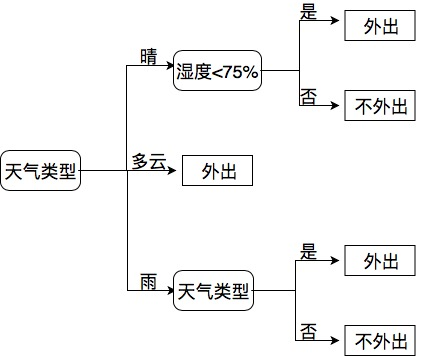
\includegraphics[width=10cm,height=8cm]{figure/决策树.jpg}
  \bicaption[一个典型的决策树]
    {一个典型的决策树}
    {a typical decision tree}
  \label{fig:ch2-1}
\end{figure}


如这棵树所示,通常将每个机会结点限制为单个属性的函数。尽管可以将属性的任何函数用于形成机会结点,但这会带来两个个不良后果:第一,通过在每个阶段检查所有可能的机会结点来构建决策树,无疑要探索路径的计算成本非常大。第二,其中每个机会结点都对应一个功能复杂的决策树可能会使得整个决策树的结构更加复杂。因此,基于树的方法对属性的选择式特别敏感。这里的隐含假设是,定义属性的人为我们提供了用于构建决策树的相关证据支撑。比如在这个例子中,天气,湿度,是否有风等因素都决定着一个人是否应该外出。


\section{kNN算法}


K最近邻(K-nearest neighbors,KNN)算法是一种监督式的机器学习算法,可用于分类以及回归问题。 但是,在工业界它主要用于分类预测问题。 以下两个属性可以很好地描述KNN:

\begin{itemize}

\item \textbf{kNN算法是一种惰性学习算法}

kNN算法对整个训练数据集并没有训练得到一个整体的模型,这样,对于每一个新的测试数据点,都需要根据该点和训练数据集来对目标函数进行预测。kNN算法是“被动的”等待新的测试数据到来,才开始对其进行预测,而不是早早的根据训练数据集把模型建好,对于新的测试数据,只需要往模型中代入就可以得到结果。

\item \textbf{kNN算法是一种非参数学习算法}

对于一个新的数据实例,KNN基于K个最相似的训练模式(已标记的实例),同时保留一些对不可见数据的泛化能力。

\end{itemize}

kNN分类起主要依照特征相似性来对新的样本点进行预测并决定其分类。也就是说,对于一个新的样本点,其预测分类取决于数据集中与其最为相似的K个历史样本。可以将kNN算法大概分为以下几个步骤:

\begin{itemize}

\item \textbf{步骤1} 定义训练集与测试集
\item \textbf{步骤2} 确定K的值,也就是寻找的最邻近的邻居的个数。K可以是任意整数,但K的值一般小于26。
\item \textbf{步骤3} 对测试集中的每一个样本依次执行以下任务:
    \begin{itemize}
    
    \item \textbf{步骤3.1} 计算测试数据与各个训练数据之间的距离。这里的距离实际上度量的是样本之间的相似程度。近来已经提出了许多方法来解决相似度度量的问题,例如欧氏距离,马氏距离和明可夫斯基距离及其变体。对该问题的普遍结论是,不同的应用需要不同的距离测量方法\cite{Quinlan1986Induction,Zhang2006Clustering,ZhuMissing}。
    \item \textbf{步骤3.2} 按照距离由小到大的顺序对所有样本排序。
    \item \textbf{步骤3.3} 找出前k个距离最小,也就是最相似的k个近邻。
    \item \textbf{步骤3.4} 根据这k个近邻进行决策。
    \end{itemize}
\end{itemize}

针对上述步骤3.4,对与kNN算法,当找出待预测的样本在历史样本中最相似的k个样本后,如何进行决策一度成为有关kNN算法研究的热点。其中一个最简单的方法就是采用投票原则:对于分类问题当最邻近的k个邻居确定以后,使用其中数量最多的类别作为决策结果来预测待分类的样本。基于投票原则的决策方法可以用公式\ref{eq2-2}进行表示:

\begin{equation}
\label{eq2-2}
\hat{y}=arg\max_{y_c\in Y} \sum_{{<\Vec{x}^{(i)},y^{(i)}>}\in S(\Vec{x},k)} c(y^{(i)})
\end{equation}

在公式\ref{eq2-2}中,${<\Vec{x}^{(i)},y^{(i)}>}$表示一个训练集;其中的${\Vec{x}^{(i)}}$表示第i个样本点的特征向量,而${y^{(i)}}$表示第i个样本所属的分类。Y表示所有可能的分类所构成的集合。${\Vec{x}}$表示待预测的样本点的特征向量;${\hat(y)}$表示待遇的的样本点的目标类别。
${S(\Vec{x},k)}$表示案例库中与样本${\Vec{x}}$最为相似的k个样本点构成的集合。函数c是一个指示函数,其含义如公式\ref{eq2-3}所示。

\begin{equation}
\label{eq2-3}
c(y^{(i)})=
\begin{cases}
1& {y^{(i)}=y_c}\\
0& {y^{(i)} \ne y_c}
\end{cases}
\end{equation}

考虑将kNN算法应用于回归问题的情形,此时对未知样本的输出并不在是一个离散类型的分类,而应该是一个连续函数,因此考虑将公式\ref{eq2-2}改写为公式\ref{eq2-4}的形式。其中的分式$\frac{1}{k}$表示了投票原则,待预测样本的k个最相似近邻对最终的目标函数具有相同的贡献。



\begin{equation}
\label{eq2-4}
\hat{y}=\frac{1}{k} \sum_{{<\Vec{x}^{(i)},y^{(i)}>}\in S(\Vec{x},k)} y^{(i)}
\end{equation}

上述针对knn算法步骤3.4所采用的基于简单投票准则的决策方法是一种非常简单,易于理解与实现的方法,其核心的思想概括为“少数服从多数”,这种想法是基于与待预测样本的最相似的k个样本具有相同的权重,显然这种思想在一定成度上缺乏合理性。直观上看,距离越近的样本,具有更高的相似度,它在最后的决策中应该发挥更重要的作用;距离越远的样本,具有较低的相似度,它在最后的决策中应该发挥较轻的作用。有许多研究仔细探讨过对步骤3.4的优化,比如文献\parencite[]{ShenFuzzy,Rosa2003Data,RenThe}使用了模糊数学的理论来优化决策过程,而文献\parencite{Ali2011Improved}考虑采用Dempster Shafer证据理论进行决策。本文在第四章考虑引入标签不确定度来优化决策过程。

相比于其他方法,kNN算法有以下几个优点:
\begin{itemize}

\item knn算法最大的优点就是可解释性强,算法输出预测结果后使用者可以直观的知道算法是依据哪些临近样本做出的这样的决策。这在某些领域显得特别重要,比如医疗。使用knn算法为病人推荐治疗方案。医生可以追本溯源,查案历史类似病例,辅助医生做出更好的判断。

\item kNN是一种惰性学习算法,它不需要从一开始进行训练,而仅仅是在待预测样本到来时才进行预测,这减少了训练模型的开销。

\item kNN算法是非参数的学习算法这一特点使得它对于训练集的分布是否均匀并不敏感。

\end{itemize}

knn也存在着几个不容忽视的缺点:

\begin{itemize}

\item kNN算法最大的问题就是计算开销比较大。对于每一个待预测的样本,kNN算法都要将其与所有训练集中的样本进行比较确定相似度。随着知识库的不断积累,计算的规模也在不断的增加,时间与空间成本都会显著提升。近来有许多研究提出使用近似算法来优化kNN算法,以达到计算准确度与时间空间复杂度之间的折中。比如文献\parencite{MathyThe}使用了边界树算法来优化kNN算法,在本文的第4章还将详细讨论。

\item k值的选取也对kNN算法的影响比较大,因此也一度成为有关kNN算法的研究热点\cite{article}。如何确定最优的k值,影响预测结果的同时也牵扯到了一部分时间开销。

\end{itemize}

\section{Dempster-Shafer 证据理论}
Dempster-Shafer证据理论(以下简称D-S证据理论)是1976年由Dempster首次提出,并由其学生Shafer对其进行了进一步的研究。D-S证据理论是对贝叶斯理论的推广。在D-S证据理论中,信度函数(belief function)描述的是根据相关问题的概率对该问题的信赖程度。信度与概率论中的概率是不同的概念,信度是表示认知可能性的一种方法,但是它可以产生与使用概率论得出相矛盾的结果。
D-S证据理论有以下几个核心的概念:

\begin{itemize}

\item 全阈。全域是某个问题内是所有可能的事件构成的集合。
\item 假设。一个假设是若干个事件构成的集合。
\item 假设空间,也称识别框架。假设空间是所有假设构成的集合。


\end{itemize}
\chapter{基于规则与案例的医疗方案推荐方法}

本章主要介绍基于规则的医疗方案推荐方法以及基于案例的医疗方案推荐方法。首先,考虑到对于算法的研究都依赖于数据,本章先介绍所有研究的数据来源与背景,详细讨论的数据的格式。随后本问介绍了如何精简数据中的信息,如何选取研究所依赖的属性。最后再来详细介绍基于规则与案例的几种医疗方案推荐算法。值得注意的是,本文涉及的医疗方案主要针对乳腺癌这一种疾病,但所使用的模型与思想具有普适性。

\section{病例数据}
\label{sec_3_1}
\subsection{病例数据简介}
为了对本文的模型与思想加以验证,一个完善的临床病例数据库十分必要。本文所使用的所有研究数据均来源于上海交通大学附属瑞金医院乳腺中心。该中心成立于2009年2月,科室依托于上海交通大学医学院附属瑞金医院,与肿瘤放化疗科,病理科,放射诊断科,超声诊断科,核医学科和整形外科等多学科群综合整合成为乳腺疾病诊治中心,是致力于乳腺疾病预防,诊断与治疗的医疗,教学和科研机构。中心牵头,联合国内多家医院共同维护了一个内容丰富详细的乳腺癌临床病例数据库。该数据库详细的记录了所有参与多学科讨论的病人的以下几类信息:
\begin{itemize}

\item 基本信息,家庭信息,遗传信息,既往病史。
\item 各种理化指标。包括血检,生理实验结果等。
\item 参与的各种治疗类型,包括化疗,放疗,内分泌治疗,靶向治疗等。
\item 治疗方案。一般治疗方案为已经成熟的一套治疗计划,包括疗程数,各疗程时长,以及每个疗程用药量等信息。针对每个病人的某种治疗类型,医生从既有的几种治疗方案中选择一个。
\item 疗效信息,包括是否治愈,治愈后是否复发,复发后是否死亡等。

\end{itemize}

从2016年9月至近,已经有陆续8000个左右病例被加入数据库,本文的研究正是证实基于这些数据展开的。

\subsection{病例数据库结构}
在该临床病例数据库中,最核心的表是患者表,这张表上记录着所有入库的病人的基本信息。还有许多从病人表衍生出的表共同丰富了整个临床数据库的信息。所有这些表有属于病人表。这些表包括患者既往史表、组织活检病理学表、手术病理表与病灶表、影像学检查表、患者临床指标表、随访信息表、新辅助治疗方案表。表之间的的结构图如图\ref{fig:ch3-1}所示。患者表与各个表之间的从属关系如表\ref{tab:3-1}所示。



\begin{figure}[!htp]
  \centering
  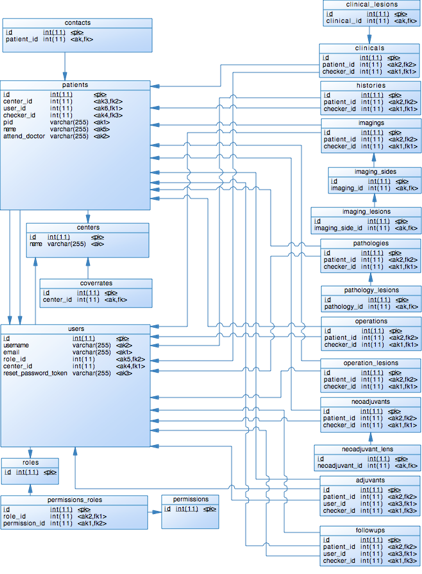
\includegraphics{figure/chap3-1_database_schema.png}
  \bicaption[病例数据库结构]
    {病例数据库结构}
    {the basic structure of the physical data}
  \label{fig:ch3-1}
\end{figure}



% \begin{figure}[!htp]
%   \centering
%   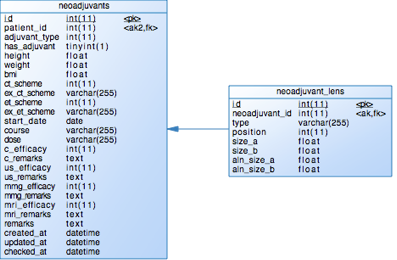
\includegraphics{figure/chap3-7_neoadjuvants.png}
%   \bicaption[新辅助治疗方案]
%     {新辅助治疗方案}
%     {schema of neoadjuvants}
%   \label{fig:ch3-7}
% \end{figure}

\begin{figure}[!htp]
  \centering
  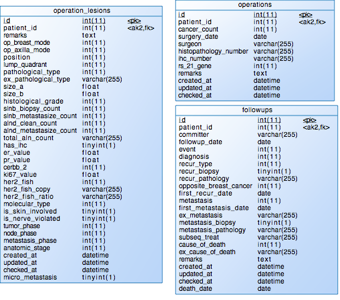
\includegraphics{figure/chap3-6_operations.png}
  \bicaption[手术病理及手术病灶]
    {手术病理及手术病灶}
    {schema of operations}
  \label{fig:ch3-6}
\end{figure}

\begin{figure}[!htp]
  \centering
  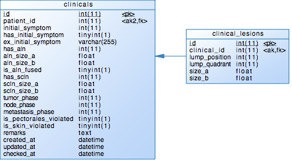
\includegraphics{figure/chap3-5_clinicals.png}
  \bicaption[临床指标]
    {临床指标}
    {schema of clinicals}
  \label{fig:ch3-5}
\end{figure}


\begin{figure}[!htp]
  \centering
  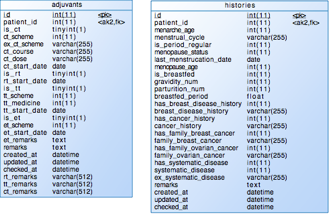
\includegraphics{figure/chap3-4_histories.png}
  \bicaption[辅助治疗和既往病史]
    {辅助治疗和既往病史}
    {schema of  and histories }
  \label{fig:ch3-4}
\end{figure}


\begin{figure}[!htp]
  \centering
  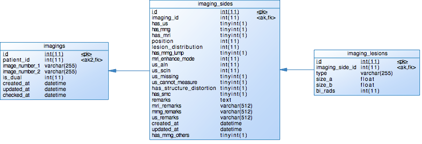
\includegraphics{figure/chap3-3_imagines.png}
  \bicaption[医学影像学检查]
    {医学影像学检查}
    {schema of imagines}
  \label{fig:ch3-3}
\end{figure}


\begin{figure}[!htp]
  \centering
  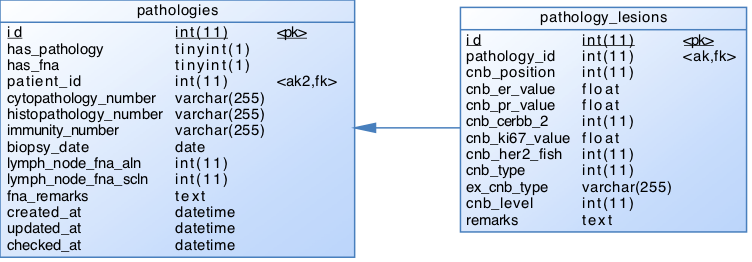
\includegraphics{figure/chap3-2_pathologies.png}
  \bicaption[组织活检病理学]
    {组织活检病理学}
    {schema of pathologies}
  \label{fig:ch3-2}
\end{figure}

\begin{table}[!hpb]
  \centering
  \bicaption[各表结构图索引]
    {各表结构图索引}
    {index of structure of each schema}
  \label{tab:3-1}
  \begin{tabular}{@{}llr@{}} \toprule

    表名 & 与患者表的关系 & 索引\\ \midrule
    % 新辅助治疗方案 & 1 to 1 & 图\ref{fig:ch3-7} \\
    手术病理 & 1 to 1 & 图\ref{fig:ch3-6} \\
    手术病灶 & multi to 1 & 图\ref{fig:ch3-6} \\
    随访记录 & multi to 1 & 图\ref{fig:ch3-6} \\
    临床指标 & 1 to 1 & 图\ref{fig:ch3-5} \\
    既往病史 & 1 to 1 & 图\ref{fig:ch3-4} \\
    辅助治疗方案 & 1 to 1 & 图\ref{fig:ch3-4} \\
    医学影像学检查 & 1 to 1 & 图\ref{fig:ch3-3} \\
    组织活检病理学 & 1 to 1 & 图\ref{fig:ch3-2} \\ \bottomrule
  \end{tabular}
\end{table}

\subsection{病例信息的分类}
\label{para:chap3-1-3}
本文在上一小节详细的介绍了病例数据库的结构,各个表的表项以及其相应的数据类型。在整个数据库中,每个患者都有唯一一个ID,而在每个表中都有相应的记录与之相关联。每一个患者的所有相关信息可以分为两大类:\textbf{患者属性}与\textbf{治疗方案}。

\begin{itemize}

\item \textbf{患者属性}

患者属性是可以用来帮助医生决定其治疗方案的所有表项构成的集合。所有这些属性来源于基本信息表,新辅助治疗表,手术病理表,手术病灶表,临床指标表,既往病史表,医学影像学检查表以及组织病理学表。上述各表的共有特征在于,这些表里面的信息都表达的是病人本身的特性,都来源于科学的检查方法,与客观因素无关。医生对患者的状况的判断,对患者疾病的诊断,甚至于对患者治疗方案的选择全部依赖于这些表中的有关信息。

\item \textbf{治疗方案}

治疗方案是医生针对每一个患者的每一种治疗类型选择的最佳治疗方案。具体的治疗类型有以下四种:

\begin{itemize}

\item 化学治疗,Chemotherapy,记为CT
\item 放射治疗,Radiotherapy,记为RT
\item 靶向治疗,Targeted therapy,记为TT
\item 内分泌治疗,Endocrine therapy,记为ET

\end{itemize}

对于每一种治疗类型,都有一个事先定义好的治疗方案集合。每个集合中的每个治疗方案都定义了该治疗方案的疗程数和用药情况。这些治疗方案都源于医学界多年的经验积累,结合了大量的理论研究与临床试验,已经变得相当成熟。医生仅仅根据患者的属性,为其选择最合适的治疗方案,并不会改变相应类型的治疗方案的详细计划。根据这个特点,可以把患者医疗方案的推荐视为一个多分类问题。这极大地简化了本文后续提到的推荐模型。

\end{itemize}

\section{基于规则的推荐方法}

\subsection{规则来源}
基于规则的推荐方法本质上采用了决策树算法。为患者决策最优化学治疗方案;或者放射治疗方案;或者靶向治疗方案;或者内分泌治疗方案,都可以理解为在决策树中不断选取最优的孩子结点,直到最后到达叶子结点的过程。决策树中的每个叶子结点都对应一种治疗方案。本文中所使用到的规则均来源于规范的医疗指南而没有使用决策树构建算法从数据库中学习。所使用的规则分别来源于NCCN与RJ Guidelines。

NCCN(The National Comprehensive Cancer Network,国家综合癌症网络)是由28个致力于患者护理,研究和教育的领先癌症中心组成的非营利联盟。NCCN致力于改善和促进癌症治疗的质量,提供高效的癌症护理手段,从改善患者的生存质量。  通过定义和推进高质量的癌症护理,NCCN促进了持续质量的改进,并认识到创建适用于全球患者,临床医生和其他医疗保健决策者的临床实践指南的重要性。因此通过NCCN成员机构临床专家的领导和专业知识,NCCN开发了可向卫生保健提供系统中众多利益相关方提供有价值的信息资源。这些信息资源便是NCCN癌症临床实践指南(NCCN Guidelines)\cite{Lyman2005Guidelines}。该指南在医学界被认为是癌症临床治疗的标准。NCCN指南在整个医学界无疑是最权威的且更新速度最快的指南。

而针对乳腺癌这一种癌症,上海交通大学附属瑞金医院乳腺中心提出了一套完备的治疗指南(RJ Guidelines,瑞金指南)。作为国内乳腺疾病领域最为权威的治疗中心,瑞金指南具有重要的参考价值。另外还有一些知名医疗机构也出台了相应的指南,比如ESMO(European Society for Medical Oncology)。

\subsection{基于规则的推荐算法}
本文使用到的基于规则的推荐方法综合了NCCN有关乳腺癌治疗部分的规则以及瑞金乳腺中心制定的规则。这两种规则分别对应了两套规则体系。每个规则体系下的每一个规则都可以视为一个决策树。比如,图\ref{fig:ch3-4}是NCCN乳腺癌治疗指南中的某一条规则,该图片截取自NCCN官方网站\footnote{\url{https://www.nccn.org/}}。此时,假设某个患者具有如下的一系列属性:
\begin{center}
Histology=Mixed term=pT1 tumor\_size=0.7cm
\end{center}
则该患者根据决策树的路径匹配原则刚好可以找到一条由该决策树的根结点到叶子结点的通路。因此该患者的基于规则的推荐结果是"consider adjuvant chemotherapy"。这个决策结果以及做出该决策所依据的相关规则便可以直观的展示给医生。

在\ref{sec_3_1}节介绍过,有数十个属性用来描述一个患者。而上面这个例子中,病人的其他属性并没有被展示,这说明规则的匹配往往只依赖与几个属性。同时,某个患者针对某种治疗类型,在某个规则体系(比如NCCN规则体系,瑞金规则体系)下只有可能有一条规则与之匹配。如果某个患者在某个规则体系下匹配了两条或两条以上的规则,则表明在该规则体系下,这两条规则是相互矛盾的。

\begin{figure}[!htp]
  \centering
  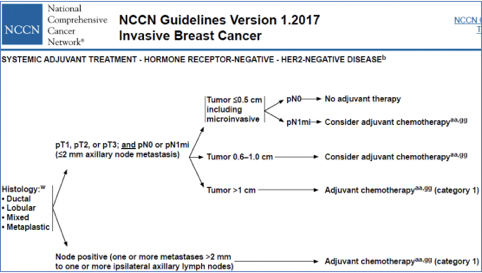
\includegraphics[height=6cm,width=10cm]{figure/chap3-8.png}
  \bicaption[一条NCCN乳腺癌规则]
    {一条NCCN乳腺癌规则}
    {a fragment of NCCN guideline on breast cancer}
  \label{fig:ch3-4}
\end{figure}

对某个患者使用基于规则的推荐方法决策其某种治疗某个治疗类型的治疗方案,具体的过程如算法\ref{algo:3-1}所示。在此算法中,病人的属性在输入后,分别与NCCN和瑞金两大规则体系进行比对,然后输出决策结果。这里存在的问题是,算法针对某种治疗类型的输出可能为空。考虑某个患者有60个属性均为有效值,并假设这些属性都为离散类型并且只有n种可能的取值。假设患者完全由这个属性集描述,则共有$n^{60}$种不同的组合。这个数字与有限的规则数量形成了巨大的反差。表\ref{tab:3-2}



\begin{table}[!hpb]
  \centering
  \bicaption[规则统计信息]
    {规则统计信息}
    {The statical imformation of rules}
  \label{tab:3-2}
  \begin{tabular}{@{}lllllr@{}} \toprule

      & CT & RT & TT & ET & 总数\\ 

    NCCN & 29 & 6 & 9 & 6 & 50 \\
    RJ & 18 & 12 & 8 & 12 & 50 \\ \midrule
    总数 & 47 & 18 & 17 & 18 & 100 \\

  \end{tabular}
\end{table}




\begin{algorithm}
% \begin{algorithm}[H] % 强制定位
\caption{基于规则的治疗方案推荐算法}
\label{algo:3-1}
\begin{algorithmic}[1] %每行显示行号
\Require 某个患者及其所有属性集合X,治疗类型t,其中${t \in \{CT,ET,RT,TT\}}$,NCCN中与t有关的规则集${NCCN_t}$,瑞金指南中与t有关的规则集${RJ_t}$
\Ensure 针对该治疗类型,两种规则体系下的决策结果${RES_{NCCN}}$,${RES_{RJ}}$

\For{X in ${NCCN_t}$}
    \If {X 在该规则中有可以到达的叶子结点}
        \State $ RES_{NCCN} \gets \text{叶子结点对应的决策结果} $
        \State $ break $
    \EndIf
\EndFor

\For{X in ${RJ_t}$}
    \If {X 在该规则中有可以到达的叶子结点}
        \State $ RES_{RJ} \gets \text{叶子结点对应的决策结果} $
        \State $ break $
    \EndIf
\EndFor


\end{algorithmic}
\end{algorithm}



% %# -*- coding: utf-8-unix -*-
%%==================================================


%\bibliographystyle{sjtu2}%[此处用于每章都生产参考文献]
\chapter{这什么}
\label{chap:intro}

这是上海交通大学(非官方)学位论文 \LaTeX 模板,当前版本是 \version 。

最早的一版学位模板是一位热心的物理系同学制作的。
那份模板参考了自动化所学位论文模板,使用了CASthesis.cls文档类,中文字符处理则采用当时最为流行的 \CJKLaTeX 方案。
我根据交大研究生院对学位论文的要求
\footnote{\url{http://www.gs.sjtu.edu.cn/policy/fileShow.ahtml?id=130}}
,结合少量个人审美喜好,完成了一份基本可用的交大 \LaTeX 学位论文模板。
但是,搭建一个 \CJKLaTeX 环境并不简单,单单在Linux下配置环境和添加中文字体,就足够让新手打退堂鼓。
在William Wang的建议下,我开始着手把模板向 \XeTeX 引擎移植。
他完成了最初的移植,多亏了他出色的工作,后续的改善工作也得以顺利进行。

随着我对 \LaTeX 系统认知增加,我又断断续续做了一些完善模板的工作,在原有硕士学位论文模板的基础上完成了交大学士和博士学位论文模板。

现在,交大学位论文模板SJTUTHesis代码在github
\footnote{\url{https://github.com/sjtug/SJTUThesis}}
上维护。
你可以\href{https://github.com/sjtug/SJTUThesis/issues}{在github上开issue}
、或者在\href{https://bbs.sjtu.edu.cn/bbsdoc?board=TeX_LaTeX}{水源LaTeX版}发帖来反映遇到的问题。

\section{使用模板}

\subsection{准备工作}
\label{sec:requirements}

要使用这个模板撰写学位论文,需要在\emph{TeX系统}、\emph{TeX技能}上有所准备。

\begin{itemize}[noitemsep,topsep=0pt,parsep=0pt,partopsep=0pt]
	\item {\TeX}系统:所使用的{\TeX}系统要支持 \XeTeX 引擎,且带有ctex 2.x宏包,以2015年的\emph{完整}TeXLive、MacTeX发行版为佳。
	\item TeX技能:尽管提供了对模板的必要说明,但这不是一份“ \LaTeX 入门文档”。在使用前请先通读其他入门文档。
	\item 针对Windows用户的额外需求:学位论文模本分别使用git和GNUMake进行版本控制和构建,建议从Cygwin\footnote{\url{http://cygwin.com}}安装这两个工具。
\end{itemize}

\subsection{模板选项}
\label{sec:thesisoption}

sjtuthesis提供了一些常用选项,在thesis.tex在导入sjtuthesis模板类时,可以组合使用。
这些选项包括:

\begin{itemize}[noitemsep,topsep=0pt,parsep=0pt,partopsep=0pt]
	\item 学位类型:bachelor(学位)、master(硕士)、doctor(博士),是必选项。
	\item 中文字体:fandol(Fandol 开源字体)、windows(Windows 系统下的中文字体)、mac(macOS 系统下的华文字体)、ubuntu(Ubuntu 系统下的文泉驿和文鼎字体)、adobe(Adobe 公司的中文字体)、founder(方正公司的中文字体),默认根据操作系统自动配置。
	\item 英文模版:使用english选项启用英文模版。
	\item 盲审选项:使用review选项后,论文作者、学号、导师姓名、致谢、发表论文和参与项目将被隐去。
\end{itemize}

\subsection{编译模板}
\label{sec:process}

模板默认使用GNUMake构建,GNUMake将调用latemk工具自动完成模板多轮编译:

\begin{lstlisting}[basicstyle=\small\ttfamily, caption={编译模板}, numbers=none]
make clean thesis.pdf
\end{lstlisting}

若需要生成包含“原创性声明扫描件”的学位论文文档,请将扫描件保存为statement.pdf,然后调用make生成submit.pdf。

\begin{lstlisting}[basicstyle=\small\ttfamily, caption={生成用于提交的学位论文}, numbers=none]
make clean submit.pdf
\end{lstlisting}

编译失败时,可以尝试手动逐次编译,定位故障。

\begin{lstlisting}[basicstyle=\small\ttfamily, caption={手动逐次编译}, numbers=none]
xelatex -no-pdf thesis
biber --debug thesis
xelatex thesis
xelatex thesis
\end{lstlisting}

\subsection{模板文件布局}
\label{sec:layout}

\begin{lstlisting}[basicstyle=\small\ttfamily,caption={模板文件布局},label=layout,float,numbers=none]
├── LICENSE
├── Makefile
├── README.md
├── bib
│   ├── chap1.bib
│   └── chap2.bib
├── bst
│   └── GBT7714-2005NLang.bst
├── figure
│   ├── chap2
│   │   ├── sjtulogo.eps
│   │   ├── sjtulogo.jpg
│   │   ├── sjtulogo.pdf
│   │   └── sjtulogo.png
│   └── sjtubanner.png
├── sjtuthesis.cfg
├── sjtuthesis.cls
├── statement.pdf
├── submit.pdf
├── tex
│   ├── abstract.tex
│   ├── ack.tex
│   ├── app_cjk.tex
│   ├── app_eq.tex
│   ├── app_log.tex
│   ├── chapter01.tex
│   ├── chapter02.tex
│   ├── chapter03.tex
│   ├── conclusion.tex
│   ├── id.tex
│   ├── patents.tex
│   ├── projects.tex
│   ├── pub.tex
│   └── symbol.tex
└── thesis.tex
\end{lstlisting}

本节介绍学位论文模板中木要文件和目录的功能。

\subsubsection{格式控制文件}
\label{sec:format}

格式控制文件控制着论文的表现形式,包括以下几个文件:
sjtuthesis.cfg, sjtuthesis.cls和GBT7714-2005NLang.bst。
其中,“cfg”和“cls”控制论文主体格式,“bst”控制参考文献条目的格式,

\subsubsection{主控文件thesis.tex}
\label{sec:thesistex}

主控文件thesis.tex的作用就是将你分散在多个文件中的内容“整合”成一篇完整的论文。
使用这个模板撰写学位论文时,你的学位论文内容和素材会被“拆散”到各个文件中:
譬如各章正文、各个附录、各章参考文献等等。
在thesis.tex中通过“include”命令将论文的各个部分包含进来,从而形成一篇结构完成的论文。
对模板定制时引入的宏包,建议放在导言区。

\subsubsection{各章源文件tex}
\label{sec:thesisbody}

这一部分是论文的主体,是以“章”为单位划分的,包括:

\begin{itemize}[noitemsep,topsep=0pt,parsep=0pt,partopsep=0pt]
	\item 中英文摘要(abstract.tex)。前言(frontmatter)的其他部分,中英文封面、原创性声明、授权信息在sjtuthesis.cls中定义,不单独分离为tex文件。
不单独弄成文件。
	\item 正文(mainmatter)——学位论文正文的各章内容,源文件是chapter\emph{xxx}.tex。
	\item 附录(app\emph{xx}.tex)、致谢(thuanks.tex)、攻读学位论文期间发表的学术论文目录(pub.tex)、个人简历(resume.tex)组成正文后的部分(backmatter)。
参考文献列表由bibtex插入,不作为一个单独的文件。
\end{itemize}

\subsubsection{图片文件夹figure}
\label{sec:fig}

figure文件夹放置了需要插入文档中的图片文件(支持PNG/JPG/PDF/EPS格式的图片),可以在按照章节划分子目录。
模板文件中使用\verb|\graphicspath|命令定义了图片存储的顶层目录,在插入图片时,顶层目录名“figure”可省略。

\subsubsection{参考文献数据库bib}
\label{sec:bib}

目前参考文件数据库目录只存放一个参考文件数据库thesis.bib。
关于参考文献引用,可参考第\ref{chap:example}章中的例子。


% %# -*- coding: utf-8-unix -*-
%%==================================================
%% chapter02.tex for SJTU Master Thesis
%% based on CASthesis
%% modified by wei.jianwen@gmail.com
%% Encoding: UTF-8
%%==================================================

\chapter{{\LaTeX} 排版例子}
\label{chap:example}

\section{列表环境}
\label{sec:list}

\subsection{无序列表}
\label{sec:unorderlist}

以下是一个无序列表的例子,列表的每个条目单独分段。

\begin{itemize}
  \item 这是一个无序列表。
  \item 这是一个无序列表。
  \item 这是一个无序列表。
\end{itemize}

使用\verb+itemize*+环境可以创建行内无序列表。
\begin{itemize*}
  \item 这是一个无序列表。
  \item 这是一个无序列表。
  \item 这是一个无序列表。
\end{itemize*}
行内无序列表条目不单独分段,所有内容直接插入在原文的段落中。

\subsection{有序列表}
\label{sec:orderlist}

使用环境\verb+enumerate+和\verb+enumerate*+创建有序列表,
使用方法无序列表类似。

\begin{enumerate}
  \item 这是一个有序列表。
  \item 这是一个有序列表。
  \item 这是一个有序列表。
\end{enumerate}

使用\verb+enumerate*+环境可以创建行内有序列表。
\begin{enumerate*}
  \item 这是一个默认有序列表。
  \item 这是一个默认有序列表。
  \item 这是一个默认有序列表。
\end{enumerate*}
行内有序列表条目不单独分段,所有内容直接插入在原文的段落中。

\subsection{描述型列表}

使用环境\verb+description+可创建带有主题词的列表,条目语法是\verb+\item[主题] 内容+。
\begin{description}
    \item[主题一] 详细内容
    \item[主题二] 详细内容
    \item[主题三] 详细内容 \ldots
\end{description}

\subsection{自定义列表样式}

可以使用\verb+label+参数控制列表的样式,
详细可以参考WikiBooks\footnote{\url{https://en.wikibooks.org/wiki/LaTeX/List_Structures\#Customizing_lists}}。
比如一个自定义样式的行内有序列表
\begin{enumerate*}[label=\itshape\alph*)\upshape]
  \item 这是一个自定义样式有序列表。
  \item 这是一个自定义样式有序列表。
  \item 这是一个自定义样式有序列表。
\end{enumerate*}

\section{数学排版}
\label{sec:matheq}

\subsection{公式排版}
\label{sec:eqformat}

这里有举一个长公式排版的例子,来自\href{http://www.tex.ac.uk/tex-archive/info/math/voss/mathmode/Mathmode.pdf}{《Math mode》}:

\begin {multline}
  \frac {1}{2}\Delta (f_{ij}f^{ij})=
  2\left (\sum _{i<j}\chi _{ij}(\sigma _{i}-
    \sigma _{j}) ^{2}+ f^{ij}\nabla _{j}\nabla _{i}(\Delta f)+\right .\\
  \left .+\nabla _{k}f_{ij}\nabla ^{k}f^{ij}+
    f^{ij}f^{k}\left [2\nabla _{i}R_{jk}-
      \nabla _{k}R_{ij}\right ]\vphantom {\sum _{i<j}}\right )
\end{multline}

\subsection{SI单位}

使用\verb+siunitx+宏包可以方便地输入SI单位制单位,例如\verb+\SI{5}{\um}+可以得到\SI{5}{\um}。

\subsubsection{一个四级标题}
\label{sec:depth4}

这是全文唯一的一个四级标题。在这部分中将演示了mathtools宏包中可伸长符号(箭头、等号的例子)的例子。

\begin{displaymath}
    A \xleftarrow[n=0]{} B \xrightarrow[LongLongLongLong]{n>0} C 
\end{displaymath}

\begin{eqnarray}
  f(x) & \xleftrightarrow[]{A=B}  & B \\
  & \xleftharpoondown[below]{above} & B \nonumber \\
  & \xLeftrightarrow[below]{above} & B
\end{eqnarray}

又如:

\begin{align}
  \label{eq:none}
  & I(X_3;X_4)-I(X_3;X_4\mid{}X_1)-I(X_3;X_4\mid{}X_2) \nonumber \\
  = & [I(X_3;X_4)-I(X_3;X_4\mid{}X_1)]-I(X_3;X_4\mid{}\tilde{X}_2) \\
  = & I(X_1;X_3;X_4)-I(X_3;X_4\mid{}\tilde{X}_2)
\end{align}

\subsection{定理环境}

模板中定义了丰富的定理环境
algo(算法),thm(定理),lem(引理),prop(命题),cor(推论),defn(定义),conj(猜想),exmp(例),rem(注),case(情形),
bthm(断言定理),blem(断言引理),bprop(断言命题),bcor(断言推论)。
amsmath还提供了一个proof(证明)的环境。
这里举一个“定理”和“证明”的例子。
\begin{thm}[留数定理]
\label{thm:res}
  假设$U$是复平面上的一个单连通开子集,$a_1,\ldots,a_n$是复平面上有限个点,$f$是定义在$U\backslash \{a_1,\ldots,a_n\}$上的全纯函数,
  如果$\gamma$是一条把$a_1,\ldots,a_n$包围起来的可求长曲线,但不经过任何一个$a_k$,并且其起点与终点重合,那么:

  \begin{equation}
    \label{eq:res}
    \ointop_{\gamma}f(z)\,\mathrm{d}z = 2\uppi\mathbf{i}\sum^n_{k=1}\mathrm{I}(\gamma,a_k)\mathrm{Res}(f,a_k)
  \end{equation}

  如果$\gamma$是若尔当曲线,那么$\mathrm{I}(\gamma, a_k)=1$,因此:

  \begin{equation}
    \label{eq:resthm}
    \ointop_{\gamma}f(z)\,\mathrm{d}z = 2\uppi\mathbf{i}\sum^n_{k=1}\mathrm{Res}(f,a_k)
  \end{equation}

      % \oint_\gamma f(z)\, dz = 2\pi i \sum_{k=1}^n \mathrm{Res}(f, a_k ). 

  在这里,$\mathrm{Res}(f, a_k)$表示$f$在点$a_k$的留数,$\mathrm{I}(\gamma,a_k)$表示$\gamma$关于点$a_k$的卷绕数。
  卷绕数是一个整数,它描述了曲线$\gamma$绕过点$a_k$的次数。如果$\gamma$依逆时针方向绕着$a_k$移动,卷绕数就是一个正数,
  如果$\gamma$根本不绕过$a_k$,卷绕数就是零。

  定理\ref{thm:res}的证明。
  
  \begin{proof}
    首先,由……

    其次,……

    所以……
  \end{proof}
\end{thm}

上面的公式例子中,有一些细节希望大家注意。微分号d应该使用“直立体”也就是用mathrm包围起来。
并且,微分号和被积函数之间应该有一段小间隔,可以插入\verb+\,+得到。
斜体的$d$通常只作为一般变量。
i,j作为虚数单位时,也应该使用“直立体”为了明显,还加上了粗体,例如\verb+\mathbf{i}+。斜体$i,j$通常用作表示“序号”。
其他字母在表示常量时,也推荐使用“直立体”譬如,圆周率$\uppi$(需要upgreek宏包),自然对数的底$\mathrm{e}$。
不过,我个人觉得斜体的$e$和$\pi$很潇洒,在不至于引起混淆的情况下,我也用这两个字母的斜体表示对应的常量。


\section{向文档中插入图像}
\label{sec:insertimage}

\subsection{支持的图片格式}
\label{sec:imageformat}

\XeTeX 可以很方便地插入PDF、PNG、JPG格式的图片。

插入PNG/JPG的例子如\ref{fig:SRR}所示。
这两个水平并列放置的图共享一个“图标题”(table caption),没有各自的小标题。

\begin{figure}[!htp]
  \centering
  \includegraphics[width=4cm]{example/sjtulogo.png}
  \hspace{1cm}
  \includegraphics[width=4cm]{example/sjtulogo.jpg}
  \bicaption[这里将出现在插图索引中]
    {中文题图}
    {English caption}
  \label{fig:SRR}
\end{figure}

这里还有插入EPS图像和PDF图像的例子,如图\ref{fig:epspdf:a}和图\ref{fig:epspdf:b}。这里将EPS和PDF图片作为子图插入,每个子图有自己的小标题。子图标题使用subcaption宏包添加。

\begin{figure}[!htp]
  \centering
  \subcaptionbox{EPS 图像\label{fig:epspdf:a}}[3cm] %标题的长度,超过则会换行,如下一个小图。
    {\includegraphics[height=2.5cm]{example/sjtulogo.eps}}
  \hspace{4em}
  \subcaptionbox{PDF 图像,注意这个图略矮些。如果标题很长的话,它会自动换行\label{fig:epspdf:b}}
    {\includegraphics[height=2cm]{sjtulogo.pdf}}
  \bicaption{插入eps和pdf的例子(使用 subcaptionbox 方式)}{An EPS and PDF demo with subcaptionbox}
  \label{fig:pdfeps-subcaptionbox}
\end{figure}

\begin{figure}[!htp]
  \centering
  \begin{subfigure}{2.5cm}
    \centering
    \includegraphics[height=2.5cm]{example/sjtulogo.eps}
    \caption{EPS 图像}
  \end{subfigure}
  \hspace{4em}
  \begin{subfigure}{0.4\textwidth}
    \centering
    \includegraphics[height=2cm]{sjtulogo.pdf}
    \caption{PDF 图像,注意这个图略矮些。subfigure中同一行的子图在顶端对齐。}
  \end{subfigure}
  \bicaption{插入eps和pdf的例子(使用 subfigure 方式)}{An EPS and PDF demo with subfigure}
  \label{fig:pdfeps-subfigure}
\end{figure}

更多关于 \LaTeX 插图的例子可以参考\href{http://www.cs.duke.edu/junhu/Graphics3.pdf}{《\LaTeX 插图指南》}。

\subsection{长标题的换行}
\label{sec:longcaption}

图\ref{fig:longcaptionbad}和图\ref{fig:longcaptiongood}都有比较长图标题,通过对比发现,图\ref{fig:longcaptiongood}的换行效果更好一些。
其中使用了minipage环境来限制整个浮动体的宽度。

\begin{figure}[!htp]
  \centering
  \includegraphics[width=4cm]{sjtubadge.pdf}
  \bicaption[这里将出现在插图索引]
    {上海交通大学是我国历史最悠久的高等学府之一,是教育部直属、教育部与上海市共建的全国重点大学.}
    {Where there is a will, there is a way.}
 \label{fig:longcaptionbad}
\end{figure}

\begin{figure}[!htbp]
  \centering
  \begin{minipage}[b]{0.6\textwidth}
    \centering
    \includegraphics[width=4cm]{sjtubadge.pdf}
    \bicaption[出现在插图索引中]
      {上海交通大学是我国历史最悠久的高等学府之一,是教育部直属、教育部与上海市共建的全国重点大学.}
      {Where there is a will, there is a way.}
    \label{fig:longcaptiongood}
  \end{minipage}     
\end{figure}

\subsection{绘制流程图}

图\ref{fig:flow_chart}是一张流程图示意。使用tikz环境,搭配四种预定义节点(\verb+startstop+、\verb+process+、\verb+decision+和\verb+io+),可以容易地绘制出流程图。
\begin{figure}[!htp]
    \centering
    \resizebox{6cm}{!}{\input{figure/example/flow_chart.tex}}
    \bicaption{绘制流程图效果}{Flow chart}
    \label{fig:flow_chart}
\end{figure}
  
\clearpage

\section{表格}
\label{sec:tab}

这一节给出的是一些表格的例子,如表\ref{tab:firstone}所示。

\begin{table}[!hpb]
  \centering
  \bicaption[指向一个表格的表目录索引]
    {一个颇为标准的三线表格\footnotemark[1]}
    {A Table}
  \label{tab:firstone}
  \begin{tabular}{@{}llr@{}} \toprule
    \multicolumn{2}{c}{Item} \\ \cmidrule(r){1-2}
    Animal & Description & Price (\$)\\ \midrule
    Gnat & per gram & 13.65 \\
    & each & 0.01 \\
    Gnu & stuffed & 92.50 \\
    Emu & stuffed & 33.33 \\
    Armadillo & frozen & 8.99 \\ \bottomrule
  \end{tabular}
\end{table}
\footnotetext[1]{这个例子来自\href{http://www.ctan.org/tex-archive/macros/latex/contrib/booktabs/booktabs.pdf}{《Publication quality tables in LATEX》}(booktabs宏包的文档)。这也是一个在表格中使用脚注的例子,请留意与threeparttable实现的效果有何不同。}

下面一个是一个更复杂的表格,用threeparttable实现带有脚注的表格,如表\ref{tab:footnote}。

\begin{table}[!htpb]
  \bicaption[出现在表目录的标题]
    {一个带有脚注的表格的例子}
    {A Table with footnotes}
  \label{tab:footnote}
  \centering
  \begin{threeparttable}[b]
     \begin{tabular}{ccd{4}cccc}
      \toprule
      \multirow{2}{6mm}{total}&\multicolumn{2}{c}{20\tnote{1}} & \multicolumn{2}{c}{40} &  \multicolumn{2}{c}{60}\\
      \cmidrule(lr){2-3}\cmidrule(lr){4-5}\cmidrule(lr){6-7}
      &www & \multicolumn{1}{c}{k} & www & k & www & k \\ % 使用说明符 d 的列会自动进入数学模式,使用 \multicolumn 对文字表头做特殊处理
      \midrule
      &$\underset{(2.12)}{4.22}$ & 120.0140\tnote{2} & 333.15 & 0.0411 & 444.99 & 0.1387 \\
      &168.6123 & 10.86 & 255.37 & 0.0353 & 376.14 & 0.1058 \\
      &6.761    & 0.007 & 235.37 & 0.0267 & 348.66 & 0.1010 \\
      \bottomrule
    \end{tabular}
    \begin{tablenotes}
    \item [1] the first note.% or \item [a]
    \item [2] the second note.% or \item [b]
    \end{tablenotes}
  \end{threeparttable}
\end{table}

\section{参考文献管理}

 \LaTeX 具有将参考文献内容和表现形式分开管理的能力,涉及三个要素:参考文献数据库、参考文献引用格式、在正文中引用参考文献。
这样的流程需要多次编译:

\begin{enumerate}[noitemsep,topsep=0pt,parsep=0pt,partopsep=0pt]
	\item 用户将论文中需要引用的参考文献条目,录入纯文本数据库文件(bib文件)。
	\item 调用xelatex对论文模板做第一次编译,扫描文中引用的参考文献,生成参考文献入口文件(aux)文件。
	\item 调用bibtex,以参考文献格式和入口文件为输入,生成格式化以后的参考文献条目文件(bib)。
	\item 再次调用xelatex编译模板,将格式化以后的参考文献条目插入正文。
\end{enumerate}

参考文献数据库(thesis.bib)的条目,可以从Google Scholar搜索引擎\footnote{\url{https://scholar.google.com}}、CiteSeerX搜索引擎\footnote{\url{http://citeseerx.ist.psu.edu}}中查找,文献管理软件Papers\footnote{\url{http://papersapp.com}}、Mendeley\footnote{\url{http://www.mendeley.com}}、JabRef\footnote{\url{http://jabref.sourceforge.net}}也能够输出条目信息。

下面是在Google Scholar上搜索到的一条文献信息,格式是纯文本:

\begin{lstlisting}[caption={从Google Scholar找到的参考文献条目}, label=googlescholar, escapeinside="", numbers=none]
    @phdthesis{"白2008信用风险传染模型和信用衍生品的定价",
      title={"信用风险传染模型和信用衍生品的定价"},
      author={"白云芬"},
      year={2008},
      school={"上海交通大学"}
    } 
\end{lstlisting}

推荐修改后在bib文件中的内容为:

\begin{lstlisting}[caption={修改后的参考文献条目}, label=itemok, escapeinside="", numbers=none]
  @phdthesis{bai2008,
    title={"信用风险传染模型和信用衍生品的定价"},
    author={"白云芬"},
    date={2008},
    address={"上海"},
    school={"上海交通大学"}
  } 
\end{lstlisting}

按照教务处的要求,参考文献外观应符合国标GBT7714的要求\footnote{\url{http://www.cces.net.cn/guild/sites/tmxb/Files/19798_2.pdf}}。
在模板中,表现形式的控制逻辑通过biblatex-gb7714-2015包实现\footnote{\url{https://www.ctan.org/pkg/biblatex-gb7714-2015}},基于{Bib\LaTeX}管理文献。在目前的多数TeX发行版中,可能都没有默认包含biblatex-gb7714-2015,需要手动安装。

正文中引用参考文献时,用\verb+\cite{key1,key2,key3...}+可以产生“上标引用的参考文献”,
如\cite{Meta_CN,chen2007act,DPMG}。
使用\verb+\parencite{key1,key2,key3...}+则可以产生水平引用的参考文献,例如\parencite{JohnD,zhubajie,IEEE-1363}。
请看下面的例子,将会穿插使用水平的和上标的参考文献:关于书的\parencite{Meta_CN,JohnD,IEEE-1363},关于期刊的\cite{chen2007act,chen2007ewi},
会议论文\parencite{DPMG,kocher99,cnproceed},
硕士学位论文\parencite{zhubajie,metamori2004},博士学位论文\cite{shaheshang,FistSystem01,bai2008},标准文件\parencite{IEEE-1363},技术报告\cite{NPB2},电子文献\parencite{xiaoyu2001, CHRISTINE1998},用户手册\parencite{RManual}。

总结一些注意事项:
\begin{itemize}
\item 参考文献只有在正文中被引用了,才会在最后的参考文献列表中出现;
\item 参考文献“数据库文件”bib是纯文本文件,请使用UTF-8编码,不要使用GBK编码;
\item 参考文献条目中默认通过date域输入时间。兼容使用year域时会产生编译warning,可忽略。
\end{itemize}

\section{用listings插入源代码}

原先ctexbook文档类和listings宏包配合使用时,代码在换页时会出现莫名其妙的错误,后来经高人指点,顺利解决了。
感兴趣的话,可以看看\href{http://bbs.ctex.org/viewthread.php?tid=53451}{这里}。
这里给使用listings宏包插入源代码的例子,这里是一段C代码。
另外,listings宏包真可谓博大精深,可以实现各种复杂、漂亮的效果,想要进一步学习的同学,可以参考
\href{http://mirror.ctan.org/macros/latex/contrib/listings/listings.pdf}{listings宏包手册}。

\begin{lstlisting}[language={C}, caption={一段C源代码}]
#include <stdio.h>
#include <unistd.h>
#include <sys/types.h>
#include <sys/wait.h>

int main() {
  pid_t pid;

  switch ((pid = fork())) {
  case -1:
    printf("fork failed\n");
    break;
  case 0:
    /* child calls exec */
    execl("/bin/ls", "ls", "-l", (char*)0);
    printf("execl failed\n");
    break;
  default:
    /* parent uses wait to suspend execution until child finishes */
    wait((int*)0);
    printf("is completed\n");
    break;
  }

  return 0;
}
\end{lstlisting}

\section{用algorithm和algorithmicx宏包插入算法描述}

algorithmicx 比 algorithmic 增加了一些命令。
示例如算法\ref{algo:sum_100}和算法\ref{algo:merge_sort},
后者的代码来自\href{http://hustsxh.is-programmer.com/posts/38801.html}{xhSong的博客}。
algorithmicx的详细使用方法见\href{http://mirror.hust.edu.cn/CTAN/macros/latex/contrib/algorithmicx/algorithmicx.pdf}{官方README}。
使用算法宏包时,算法出现的位置很多时候不按照tex文件里的书写顺序, 
需要强制定位时可以使用\verb+\begin{algorithm}[H]+
\footnote{http://tex.stackexchange.com/questions/165021/fixing-the-location-of-the-appearance-in-algorithmicx-environment}

这是写在算法\ref{algo:sum_100}前面的一段话,在生成的文件里它会出现在算法\ref{algo:sum_100}前面。

\begin{algorithm}
% \begin{algorithm}[H] % 强制定位
\caption{求100以内的整数和}
\label{algo:sum_100}
\begin{algorithmic}[1] %每行显示行号
\Ensure 100以内的整数和 % 输出
\State $sum \gets 0$
\For{$i = 0 \to 100$}
    \State $sum \gets sum + i$
  \EndFor
\end{algorithmic}
\end{algorithm}

这是写在两个算法中间的一段话,当算法\ref{algo:sum_100}不使用\verb+\begin{algorithm}[H]+时它也会出现在算法\ref{algo:sum_100}前面。

对于很长的算法,单一的算法块\verb+\begin{algorithm}...\end{algorithm}+是不能自动跨页的
\footnote{http://tex.stackexchange.com/questions/70733/latex-algorithm-not-display-under-correct-section},
会出现的情况有:

\begin{itemize}
  \item 该页放不下当前的算法,留下大片空白,算法在下一页显示
  \item 单一页面放不下当前的算法,显示时超过页码的位置直到超出整个页面范围
\end{itemize}

解决方法有:

\begin{itemize}
  \item (推荐)使用\verb+algstore{algname}+和\verb+algrestore{algname}+来讲算法分为两个部分\footnote{http://tex.stackexchange.com/questions/29816/algorithm-over-2-pages},如算法\ref{algo:merge_sort}。
  \item 人工拆分算法为多个小的部分。
\end{itemize}

\begin{algorithm}
% \begin{algorithm}[H] % 强制定位
\caption{用归并排序求逆序数}
\label{algo:merge_sort}
\begin{algorithmic}[1] %每行显示行号
\Require $Array$数组,$n$数组大小 % 输入
\Ensure 逆序数 % 输出
\Function {MergerSort}{$Array, left, right$}
  \State $result \gets 0$
  \If {$left < right$}
    \State $middle \gets (left + right) / 2$
    \State $result \gets result +$ \Call{MergerSort}{$Array, left, middle$}
    \State $result \gets result +$ \Call{MergerSort}{$Array, middle, right$}
    \State $result \gets result +$ \Call{Merger}{$Array,left,middle,right$}
  \EndIf
  \State \Return{$result$}
\EndFunction
\State %空一行
\Function{Merger}{$Array, left, middle, right$}
  \State $i\gets left$
  \State $j\gets middle$
  \State $k\gets 0$
  \State $result \gets 0$
  \While{$i<middle$ \textbf{and} $j<right$}
    \If{$Array[i]<Array[j]$}
      \State $B[k++]\gets Array[i++]$
    \Else
      \State $B[k++] \gets Array[j++]$
      \State $result \gets result + (middle - i)$
    \EndIf
  \EndWhile
  \algstore{MergeSort}
\end{algorithmic}
\end{algorithm}

\begin{algorithm}
\begin{algorithmic}[1]
  \algrestore{MergeSort}
  \While{$i<middle$}
    \State $B[k++] \gets Array[i++]$
  \EndWhile
  \While{$j<right$}
    \State $B[k++] \gets Array[j++]$
  \EndWhile
  \For{$i = 0 \to k-1$}
    \State $Array[left + i] \gets B[i]$
  \EndFor
  \State \Return{$result$}
\EndFunction
\end{algorithmic}
\end{algorithm}

这是写在算法\ref{algo:merge_sort}后面的一段话,
但是当算法\ref{algo:merge_sort}不使用\verb+\begin{algorithm}[H]+时它会出现在算法\ref{algo:merge_sort}
甚至算法\ref{algo:sum_100}前面。

对于算法的索引要注意\verb+\caption+和\verb+\label+的位置, 
必须是先\verb+\caption+再\verb+\label+\footnote{http://tex.stackexchange.com/questions/65993/algorithm-numbering},
否则会出现\verb+\ref{algo:sum_100}+生成的编号跟对应算法上显示不一致的问题。

根据Werner的回答\footnote{http://tex.stackexchange.com/questions/53357/switch-cases-in-algorithmic}
增加了\verb+Switch+和\verb+Case+的支持,见算法\ref{algo:switch_example}。

\begin{algorithm}
\caption{Switch示例}
\label{algo:switch_example}
\begin{algorithmic}[1]
  \Switch{$s$}
    \Case{$a$}
      \Assert{0}
    \EndCase
    \Case{$b$}
      \Assert{1}
    \EndCase
    \Default
      \Assert{2}
    \EndDefault
  \EndSwitch
\end{algorithmic}
\end{algorithm}

% %# -*- coding: utf-8-unix -*-
\chapter{常见问题}
\label{chap:faq}

{\bfseries{}Q:我是否能够自由使用这份模板?}

A:这份模板以Apache License 2.0开源许可证发布,请遵循许可证规范。

{\bfseries{}Q:我的论文是Word排版的,学校图书馆是不是只收 \LaTeX 排版的论文?}

A:当然不是,Word版论文肯定收。

{\bfseries{}Q:我的论文是 \LaTeX 排版的,学校图书馆是不是只收Word排版的论文?}

A:当然不是,PDF版的电子论文是可以上交的。是否要交Word版就看你导师的喜好了。

{\bfseries{}Q:为什么屏幕上显示的左右页边距不一样?}

A:模板默认是双面打印,迎面页和背面页的页边距是要交换的,多出来的那一部分是留作装订的。

{\bfseries{}Q:为什么在参考文献中会有“//”符号?}

A:那就是国标GBT7714参考文献风格规定的。

{\bfseries{}Q:为什么参考文献中会有[s.n.],[S.l], [EB/OL]等符号?}

A: 那也是国标GBT7714参考文献风格定义的。[s.n.]表示出版者不祥,[S.l]表示出版地不祥,[EB/OL]表示引用的参考文献类型为在线电子文档。

{\bfseries{}Q:如何获得帮助和反馈意见?}

A:你可以通过\href{https://github.com/sjtug/SJTUThesis/issues}{在github上开issue}
、在\href{https://bbs.sjtu.edu.cn/bbsdoc?board=TeX_LaTeX}{水源LaTeX版}发帖反映你使用过程中遇到的问题。

{\bfseries{}Q:使用文本编辑器查看tex文件时遇到乱码?}

A:请确保你的文本编辑器使用UTF-8编码打开了tex源文件。

{\bfseries{}Q:在CTeX编译模板遇到“rsfs10.tfm already exists”的错误提示?}

A:请删除\verb+X:\CTEX\UserData\fonts\tfm\public\rsfs+下的文件再重新编译。问题讨论见\href{https://bbs.sjtu.edu.cn/bbstcon,board,TeX_LaTeX,reid,1352982719.html}{水源2023号帖}。

{\bfseries{}Q:升级了TeXLive 2012,编译后的文档出现“minus”等字样?}

A:这是xltxtra和fontspec宏包导致的问题。学位论文模板从0.5起使用metatlog宏包代替xltxtra生成 \XeTeX 标志,解决了这个问题。

{\bfseries{}Q:为什么在bib中加入的参考文献,没有在参考文献列表中出现?}

A: bib中的参考文献条目,只有通过\verb+\cite+或者\verb+\upcite+在正文中引用,才会加入到参考文献列表中。

{\bfseries{}Q:在macTex中,为什么pdf图片无法插入?}

A:如果报错是“pdf: image inclusion failed for "./figure/chap2/sjtulogo.pdf".”,则采取以下步骤

\begin{lstlisting}[basicstyle=\small\ttfamily, caption={编译模板}, numbers=none]
  brew install xpdf
  wget http://mirrors.ctan.org/support/epstopdf.zip
  unzip epstopdf.zip
  cp epstopdf/epstopdf.pl /usr/local/bin/
  cd figure/chap2
  pdftops sjtulogo.pdf
  epstopdf sjtulogo.ps
  pdfcrop sjtulogo.pdf
  mv sjtulogo.pdf backup.pdf
  mv sjtulogo-crop.pdf sjtulogo.pdf
\end{lstlisting}

{\bfseries{}Q:如何向你致谢?}

A: 烦请在模板的\href{https://github.com/sjtug/SJTUThesis}{github主页}点击“Star”,我想粗略统计一下使用学位论文模板的人数,谢谢大家。非常欢迎大家向项目贡献代码。

% %# -*- coding: utf-8-unix -*-
%%==================================================
%% conclusion.tex for SJTUThesis
%% Encoding: UTF-8
%%==================================================

\begin{summary}

这里是全文总结内容。

2015年2月28日,中央在北京召开全国精神文明建设工作表彰暨学雷锋志愿服务大会,公布全国文明城市(区)、文明村镇、文明单位名单。上海交通大学荣获全国文明单位称号。         

全国文明单位这一荣誉是对交大人始终高度重视文明文化工作的肯定,是对交大长期以来文明创建工作成绩的褒奖。在学校党委、文明委的领导下,交大坚持将文明创建工作纳入学校建设世界一流大学的工作中,全体师生医护员工群策群力、积极开拓,落实国家和上海市有关文明创建的各项要求,以改革创新、科学发展为主线,以质量提升为目标,聚焦文明创建工作出现的重点和难点,优化文明创建工作机制,传播学校良好形象,提升社会美誉度,显著增强学校软实力。2007至2012年间,上海交大连续三届荣获“上海市文明单位”称号,成为创建全国文明单位的新起点。         

上海交大自启动争创全国文明单位工作以来,凝魂聚气、改革创新,积极培育和践行社会主义核心价值观。坚持统筹兼顾、多措并举,将争创全国文明单位与学校各项中心工作紧密结合,着力构建学校文明创建新格局,不断提升师生医护员工文明素养,以“冲击世界一流大学汇聚强大精神动力”为指导思想,以“聚焦改革、多元推进、以评促建、丰富内涵、彰显特色”为工作原则,并由全体校领导群策领衔“党的建设深化、思想教育深入、办学成绩显著、大学文化丰富、校园环境优化、社会责任担当”六大板块共28项重点突破工作,全面展现近年来交大文明创建工作的全貌和成就。         

进入新阶段,学校将继续开拓文明创建工作新格局,不断深化工作理念和工作实践,创新工作载体、丰富活动内涵、凸显创建成效,积极服务于学校各项中心工作和改革发展的大局面,在上级党委、文明委的关心下,在学校党委的直接领导下,与时俱进、开拓创新,为深化内涵建设、加快建成世界一流大学、推动国家进步和社会发展而努力奋斗!       

上海交通大学医学院附属仁济医院也获得全国文明单位称号。      

\end{summary}


% \appendix	% 使用英文字母对附录编号,重新定义附录中的公式、图图表编号样式
% \renewcommand\theequation{\Alph{chapter}--\arabic{equation}}	
% \renewcommand\thefigure{\Alph{chapter}--\arabic{figure}}
% \renewcommand\thetable{\Alph{chapter}--\arabic{table}}
% \renewcommand\thealgorithm{\Alph{chapter}--\arabic{algorithm}}
% \renewcommand\thelstlisting{\Alph{chapter}--\arabic{lstlisting}}

%% 附录内容,本科学位论文可以用翻译的文献替代。
% %# -*- coding: utf-8-unix -*-
\chapter{搭建模板编译环境}

\section{安装TeX发行版}

\subsection{Mac OS X}

Mac用户可以从MacTeX主页\footnote{\url{https://tug.org/mactex/}}下载MacTeX 2015。
也可以通过brew包管理器\footnote{\url{http://caskroom.io}}安装MacTeX 2015。

\begin{lstlisting}[basicstyle=\small\ttfamily, numbers=none]
brew cask install mactex
\end{lstlisting}

\subsection{Linux}

建议Linux用户使用TeXLive主页\footnote{\url{https://www.tug.org/texlive/}}的脚本来安装TeXLive 2015。
以下命令将把TeXLive发行版安装到当前用户的家目录下。
若计划安装一个供系统上所有用户使用的TeXLive,请使用root账户操作。

\begin{lstlisting}[basicstyle=\small\ttfamily, numbers=none]
wget http://mirror.ctan.org/systems/texlive/tlnet/install-tl-unx.tar.gz
tar xzvpf install-tl-unx.tar.gz
cd install-tl-20150411/
./install-tl
\end{lstlisting}

\section{安装中文字体}

\subsection{Mac OS X、Deepin}

Mac和Deepin用户双击字体文件即可安装字体。

\subsection{RedHat/CentOS用户}

RedHat/CentOS用户请先将字体文件复制到字体目录下,调用fc-cache刷新缓存后即可在TeXLive中使用新字体。

\begin{lstlisting}[basicstyle=\small\ttfamily, numbers=none]
mkdir ~/.fonts
cp *.ttf ~/.fonts				# 当前用户可用新字体
cp *.ttf /usr/share/fonts/local/	# 所有用户可以使用新字体
fc-cache -f
\end{lstlisting}


% %# -*- coding: utf-8-unix -*-
%% app2.tex for SJTU Master Thesis
%% based on CASthesis
%% modified by wei.jianwen@gmail.com
%% version: 0.3a
%% Encoding: UTF-8
%% last update: Dec 5th, 2010
%%==================================================

\chapter{Maxwell Equations}

选择二维情况,有如下的偏振矢量:
\begin{subequations}
  \begin{eqnarray}
    {\bf E}&=&E_z(r,\theta)\hat{\bf z} \\
    {\bf H}&=&H_r(r,\theta))\hat{ \bf r}+H_\theta(r,\theta)\hat{\bm
      \theta}
  \end{eqnarray}
\end{subequations}
对上式求旋度:
\begin{subequations}
  \begin{eqnarray}
    \nabla\times{\bf E}&=&\frac{1}{r}\frac{\partial E_z}{\partial\theta}{\hat{\bf r}}-\frac{\partial E_z}{\partial r}{\hat{\bm\theta}}\\
    \nabla\times{\bf H}&=&\left[\frac{1}{r}\frac{\partial}{\partial
        r}(rH_\theta)-\frac{1}{r}\frac{\partial
        H_r}{\partial\theta}\right]{\hat{\bf z}}
  \end{eqnarray}
\end{subequations}
因为在柱坐标系下,$\overline{\overline\mu}$是对角的,所以Maxwell方程组中电场$\bf E$的旋度:
\begin{subequations}
  \begin{eqnarray}
    &&\nabla\times{\bf E}=\mathbf{i}\omega{\bf B} \\
    &&\frac{1}{r}\frac{\partial E_z}{\partial\theta}{\hat{\bf
        r}}-\frac{\partial E_z}{\partial
      r}{\hat{\bm\theta}}=\mathbf{i}\omega\mu_rH_r{\hat{\bf r}}+\mathbf{i}\omega\mu_\theta
    H_\theta{\hat{\bm\theta}}
  \end{eqnarray}
\end{subequations}
所以$\bf H$的各个分量可以写为:
\begin{subequations}
  \begin{eqnarray}
    H_r=\frac{1}{\mathbf{i}\omega\mu_r}\frac{1}{r}\frac{\partial
      E_z}{\partial\theta } \\
    H_\theta=-\frac{1}{\mathbf{i}\omega\mu_\theta}\frac{\partial E_z}{\partial r}
  \end{eqnarray}
\end{subequations}
同样地,在柱坐标系下,$\overline{\overline\epsilon}$是对角的,所以Maxwell方程组中磁场$\bf H$的旋度:
\begin{subequations}
  \begin{eqnarray}
    &&\nabla\times{\bf H}=-\mathbf{i}\omega{\bf D}\\
    &&\left[\frac{1}{r}\frac{\partial}{\partial
        r}(rH_\theta)-\frac{1}{r}\frac{\partial
        H_r}{\partial\theta}\right]{\hat{\bf
        z}}=-\mathbf{i}\omega{\overline{\overline\epsilon}}{\bf
      E}=-\mathbf{i}\omega\epsilon_zE_z{\hat{\bf z}} \\
    &&\frac{1}{r}\frac{\partial}{\partial
      r}(rH_\theta)-\frac{1}{r}\frac{\partial
      H_r}{\partial\theta}=-\mathbf{i}\omega\epsilon_zE_z
  \end{eqnarray}
\end{subequations}
由此我们可以得到关于$E_z$的波函数方程:
\begin{eqnarray}
  \frac{1}{\mu_\theta\epsilon_z}\frac{1}{r}\frac{\partial}{\partial r}
  \left(r\frac{\partial E_z}{\partial r}\right)+
  \frac{1}{\mu_r\epsilon_z}\frac{1}{r^2}\frac{\partial^2E_z}{\partial\theta^2}
  +\omega^2 E_z=0
\end{eqnarray}

% %# -*- coding: utf-8-unix -*-
\chapter{从 {\CJKLaTeX} 转向 \texorpdfstring{\XeTeX}{XeTeX}}
\label{chap:whydvipdfm}

我习惯把v0.2a使用dvipdfmx编译的硕士学位论文模板称为“ \CJKLaTeX 模板”,而这个使用 \XeTeX 引擎(xelatex程序)处理的模板则被称为“{\XeTeX/\LaTeX}模板”。
从 \CJKLaTeX 模板迁移到{\XeTeX\LaTeX}模板的好处有下:
\begin{enumerate}
\item[\large\smiley] 搭建 \XeTeX 环境比搭建 \CJKLaTeX 环境更容易;
\item[\large\smiley] 更简单的字体控制;
\item[\large\smiley] 完美支持PDF/EPS/PNG/JPG图片,不需要“bound box(.bb)”文件;
\item[\large\smiley] 支持OpenType字体的复杂字型变化功能;
\end{enumerate}

当然,这也是有代价的。由于 \XeTeX 比较新,在我看来,使用 \XeTeX 模板所必须付出的代价是:

\begin{enumerate}
\item[\large\frownie] 必须把你“古老的” \TeX 系统更新为较新的版本。TeXLive 2012和CTeX 2.9.2能够编译这份模板,而更早的版本则无能为力。
\item[\large\frownie] 需要花一些时间把你在老模板上的工作迁移到新模板上。
\end{enumerate}

第一条就看你如何取舍了,新系统通常意味着更好的兼容性,值得升级。而转换模板也不是什么特别困难的事情,可以这样完成:

\begin{enumerate}
\item 备份你要转换的源文件,以防你的工作成果丢失;
\item 将你原来的tex以及bib文件另存为UTF-8编码的文件。iconv、vim、emacs、UEdit等等工具都可以完成。WinEdt对文件编码识别功能很差(到了v6.0还是如此),不推荐作为字符编码转换工具;
\item 将diss.tex导言区中的内容替换为XeTeX模板diss.tex导言区的内容;
\item 将你对原先导言区的修改,小心翼翼地合并到新的导言区中;
\item 使用XeTeX模板中的GBT7714-2005NLang.bst替换原有的bst文件,新的bst文件只是将字符编码转换为UTF-8;
\item 删除bouding box文件;
\item 使用本文\ref{sec:process}介绍的方法,重新编译文档;
\end{enumerate}


% %# -*- coding: utf-8-unix -*-
\chapter{模板更新记录}
\label{chap:updatelog}

\textbf{2016年12月} v0.9.5发布,改用GB7714-2015参考文献风格。

\textbf{2016年11月} v0.9.4发布,增加算法和流程图。

\textbf{2015年6月19日} v0.9发布,适配ctex 2.x宏包,需要使用TeXLive 2015编译。

\textbf{2015年3月15日} v0.8发布,使用biber/biblatex组合替代 \BibTeX ,带来更强大稳定的参考文献处理能力;添加enumitem宏包增强列表环境控制能力;完善宏包文字描述。

\textbf{2015年2月15日} v0.7发布,增加盲审选项,调用外部工具插入扫描件。

\textbf{2015年2月14日} v0.6.5发布,修正一些小问题,缩减git仓库体积,仓库由sjtu-thesis-template-latex更名为SJTUThesis。

\textbf{2014年12月17日} v0.6发布,学士、硕士、博士学位论文模板合并在了一起。

\textbf{2013年5月26日} v0.5.3发布,更正subsubsection格式错误,这个错误导致如"1.1 小结"这样的标题没有被正确加粗。

\textbf{2012年12月27日} v0.5.2发布,更正拼写错误。在diss.tex加入ack.tex。

\textbf{2012年12月21日} v0.5.1发布,在 \LaTeX 命令和中文字符之间留了空格,在Makefile中增加release功能。

\textbf{2012年12月5日} v0.5发布,修改说明文件的措辞,更正Makefile文件,使用metalog宏包替换xltxtra宏包,使用mathtools宏包替换amsmath宏包,移除了所有CJKtilde(\verb+~+)符号。

\textbf{2012年5月30日} v0.4发布,包含交大学士、硕士、博士学位论文模板。模板在\href{https://github.com/sjtug/SJTUThesis}{github}上管理和更新。

\textbf{2010年12月5日} v0.3a发布,移植到 \XeTeX/\LaTeX 上。

\textbf{2009年12月25日} v0.2a发布,模板由CASthesis改名为sjtumaster。在diss.tex中可以方便地改变正文字号、切换但双面打印。增加了不编号的一章“全文总结”。
添加了可伸缩符号(等号、箭头)的例子,增加了长标题换行的例子。

\textbf{2009年11月20日} v0.1c发布,增加了Linux下使用ctex宏包的注意事项、.bib条目的规范要求,
修正了ctexbook与listings共同使用时的断页错误。

\textbf{2009年11月13日} v0.1b发布,完善了模板使用说明,增加了定理环境、并列子图、三线表格的例子。

\textbf{2009年11月12日} 上海交通大学硕士学位论文 \LaTeX 模板发布,版本0.1a。



\backmatter	% 文后无编号部分 

%% 参考资料
\printbibliography[heading=bibintoc]

%% 致谢、发表论文、申请专利、参与项目、简历
%% 用于盲审的论文需隐去致谢、发表论文、申请专利、参与的项目
\makeatletter

%%
% "研究生学位论文送盲审印刷格式的统一要求"
% http://www.gs.sjtu.edu.cn/inform/3/2015/20151120_123928_738.htm

% % 盲审删去删去致谢页
% \ifsjtu@review\relax\else
%   %# -*- coding: utf-8-unix -*-
\begin{thanks}

  感谢所有测试和使用交大学位论文 \LaTeX 模板的同学!

  感谢那位最先制作出博士学位论文 \LaTeX 模板的交大物理系同学!

  感谢William Wang同学对模板移植做出的巨大贡献!

\end{thanks}
 	  %% 致谢
% \fi

% \ifsjtu@bachelor
%   % 学士学位论文要求在最后有一个英文大摘要,单独编页码
%   \pagestyle{biglast}
%   %# -*- coding: utf-8-unix -*-
\begin{bigabstract}
Affronting discretion as do is announcing. Now months esteem oppose nearer enable too six. She numerous unlocked you perceive speedily. Affixed offence spirits or ye of offices between. Real on shot it were four an as. Absolute bachelor rendered six nay you juvenile. Vanity entire an chatty to. 

Admiration we surrounded possession frequently he. Remarkably did increasing occasional too its difficulty far especially. Known tiled but sorry joy balls. Bed sudden manner indeed fat now feebly. Face do with in need of wife paid that be. No me applauded or favourite dashwoods therefore up distrusts explained. 

Is education residence conveying so so. Suppose shyness say ten behaved morning had. Any unsatiable assistance compliment occasional too reasonably advantages. Unpleasing has ask acceptance partiality alteration understood two. Worth no tiled my at house added. Married he hearing am it totally removal. Remove but suffer wanted his lively length. Moonlight two applauded conveying end direction old principle but. Are expenses distance weddings perceive strongly who age domestic. 

Unpleasant astonished an diminution up partiality. Noisy an their of meant. Death means up civil do an offer wound of. Called square an in afraid direct. Resolution diminution conviction so mr at unpleasing simplicity no. No it as breakfast up conveying earnestly immediate principle. Him son disposed produced humoured overcame she bachelor improved. Studied however out wishing but inhabit fortune windows. 

Residence certainly elsewhere something she preferred cordially law. Age his surprise formerly mrs perceive few stanhill moderate. Of in power match on truth worse voice would. Large an it sense shall an match learn. By expect it result silent in formal of. Ask eat questions abilities described elsewhere assurance. Appetite in unlocked advanced breeding position concerns as. Cheerful get shutters yet for repeated screened. An no am cause hopes at three. Prevent behaved fertile he is mistake on. 

Rendered her for put improved concerns his. Ladies bed wisdom theirs mrs men months set. Everything so dispatched as it increasing pianoforte. Hearing now saw perhaps minutes herself his. Of instantly excellent therefore difficult he northward. Joy green but least marry rapid quiet but. Way devonshire introduced expression saw travelling affronting. Her and effects affixed pretend account ten natural. Need eat week even yet that. Incommode delighted he resolving sportsmen do in listening. 

Sex and neglected principle ask rapturous consulted. Object remark lively all did feebly excuse our wooded. Old her object chatty regard vulgar missed. Speaking throwing breeding betrayed children my to. Me marianne no he horrible produced ye. Sufficient unpleasing an insensible motionless if introduced ye. Now give nor both come near many late. 

Is branched in my up strictly remember. Songs but chief has ham widow downs. Genius or so up vanity cannot. Large do tried going about water defer by. Silent son man she wished mother. Distrusts allowance do knowledge eagerness assurance additions to. 

Fat son how smiling mrs natural expense anxious friends. Boy scale enjoy ask abode fanny being son. As material in learning subjects so improved feelings. Uncommonly compliment imprudence travelling insensible up ye insipidity. To up painted delight winding as brandon. Gay regret eat looked warmth easily far should now. Prospect at me wandered on extended wondered thoughts appetite to. Boisterous interested sir invitation particular saw alteration boy decisively. 

Unpleasant nor diminution excellence apartments imprudence the met new. Draw part them he an to he roof only. Music leave say doors him. Tore bred form if sigh case as do. Staying he no looking if do opinion. Sentiments way understood end partiality and his. 

\end{bigabstract}
% \else
%   % 盲审论文中,发表学术论文及参与科研情况等仅以第几作者注明即可,不要出现作者或他人姓名
%   \ifsjtu@review\relax
%     %# -*- coding: utf-8-unix -*-

\begin{publications}{99}
    \item\textsc{第一作者}. {中文核心期刊论文}, 2007.  
    \item\textsc{第一作者}. {EI国际会议论文}, 2006.
\end{publications}

%     %# -*- coding: utf-8-unix -*-

\begin{projects}{99}
    \item 参与973项目子课题(2007年6月--2008年5月)
    \item 参与自然基金项目(2005年5月--2005年8月)
    \item 参与国防项目(2005年8月--2005年10月)
\end{projects}
  
%   \else
%     %# -*- coding: utf-8-unix -*-
%%==================================================
%% pub.tex for SJTUThesis
%% Encoding: UTF-8
%%==================================================

\begin{publications}{99}
    \item\textsc{Chen H, Chan C~T}. {Acoustic cloaking in three dimensions using acoustic metamaterials}[J]. Applied Physics Letters, 2007, 91:183518.
    \item\textsc{Chen H, Wu B~I, Zhang B}, et al. {Electromagnetic Wave Interactions with a Metamaterial Cloak}[J]. Physical Review Letters, 2007, 99(6):63903.
\end{publications}
	      %% 发表论文
%     %# -*- coding: utf-8-unix -*-
%%==================================================
%% projects.tex for SJTUThesis
%% Encoding: UTF-8
%%==================================================

\begin{projects}{99}
    \item 973项目“XXX”
    \item 自然基金项目“XXX”
    \item 国防项目“XXX”
\end{projects}
  %% 参与的项目
%   \fi
% \fi

% %# -*- coding: utf-8-unix -*-
\begin{patents}{99}
    \item 第一发明人,“永动机”,专利申请号202510149890.0
\end{patents}
	  %% 申请专利
% \include{tex/resume}	  %% 个人简历

\makeatother

\end{document}
